%  Big Data and Cognitive Computing (MDPI) — submission draft
\documentclass[journal,article,submit,pdftex,moreauthors]{Definitions/mdpi}

\firstpage{1}
\makeatletter\setcounter{page}{\@firstpage}\makeatother
\pubvolume{1}\issuenum{1}\articlenumber{0}\pubyear{2026}\copyrightyear{2026}
\datereceived{ }\daterevised{ }\dateaccepted{ }\datepublished{ }

%=================================================================
\Title{Algorithmic Diffusion on YouTube: A Machine Learning Analysis of
Channel-Level Information Spread and Its Cross-Platform Generalisability}

\newcommand{\orcidauthorA}{0000-0000-0000-000X}
\newcommand{\orcidauthorB}{0000-0000-0000-000X}

\Author{Kamila Bakenova $^{1}$\orcidA{},
        Oleksandr Kuznetsov $^{2,3,}$*\orcidB{},
        Aigul Shaikhanova $^{1}$,
        Davyd Cherkaskyi $^{1}$,
        Borys Khrushkov $^{1}$ and
        Valentyn Chernushevych $^{1}$}

\AuthorNames{Kamila Bakenova, Oleksandr Kuznetsov, Aigul Shaikhanova,
             Davyd Cherkaskyi, Borys Khrushkov, Valentyn Chernushevych}

\address{%
$^{1}$\quad Department of Information Security, L.N.~Gumilyov Eurasian National
University, Satpayev~2, Astana 010008, Kazakhstan\\
$^{2}$\quad Department of Theoretical and Applied Sciences, eCampus University,
Via Isimbardi~10, 22060 Novedrate, Italy\\
$^{3}$\quad Department of Intelligent Software Systems and Technologies,
V.N.~Karazin Kharkiv National University, 4 Svobody Sq., 61022 Kharkiv, Ukraine}

\corres{Correspondence: oleksandr.kuznetsov@uniecampus.it}

%=================================================================
\abstract{%
(1)~Background: Information diffusion models developed for graph-based
platforms such as Reddit and broadcast architectures such as Telegram
identify temporal features---particularly the timing of peak spread---as
dominant predictors of coverage.
Whether these predictors generalise to platforms where content is
distributed through algorithmic recommendation rather than social-graph
contagion remains an open question.
(2)~Methods: We analyse the YouNiverse dataset~\cite{ref-ribeiro2021},
comprising 133,364 English-language YouTube channels observed weekly from
January~2015 to September~2019 (18.9~million observations).
We derive channel-level diffusion features---including time-to-peak,
post-peak decay rate, diffusion volatility, and upload frequency---and
train three machine learning models (Linear Regression, Random~Forest,
and LightGBM) on two tasks: predicting peak weekly view growth (regression)
and identifying viral channels (classification).
A single-feature naive baseline (subscriber count alone) establishes the
marginal contribution of temporal and behavioural features, and a temporal
split experiment (training on channels peaking before~2018, testing on
2018--2019) assesses robustness to temporal ordering.
(3)~Results: LightGBM achieves $R^2 = 0.776$ (5-fold CV:
$0.778 \pm 0.003$) compared with $R^2 = 0.548$ for the naive baseline,
a net gain of $+0.228~R^2$.
SHAP analysis identifies subscriber rank as the dominant predictor
(29.3\% of total attribution), while time-to-peak ranks fourteenth
(1.1\%), in contrast to its dominant role on Reddit ($r = 0.995$,
rank~\#1~\cite{ref-paper1}).
For virality classification, LightGBM achieves ROC-AUC~$= 0.967$.
Under the temporal split, Random~Forest ($R^2 = 0.703$) outperforms
LightGBM ($R^2 = 0.683$), indicating that more conservative ensemble
models provide better cross-temporal robustness.
(4)~Conclusions: Algorithmic recommendation decouples temporal diffusion
dynamics from coverage magnitude, rendering time-to-peak uninformative
on YouTube.
Platform architecture fundamentally constrains the generalisability of
diffusion predictors, and platform-specific models are required.%
}

\keyword{information diffusion; YouTube; machine learning; LightGBM; Random Forest;
         SHAP; time-to-peak; platform architecture; channel-level analysis;
         temporal validation; viral content; social media analytics; Big Data}

%=================================================================
\begin{document}

%=================================================================
\section{Introduction}
\label{sec:intro}

The study of information diffusion in social media has produced a substantial
body of models grounded in the assumption that spread follows the logic of
social contagion: content propagates through network ties, and the speed of
early propagation is a reliable predictor of eventual reach
\cite{ref-kermack1927,ref-pastor2015,ref-goel2016}.
This assumption has been validated empirically on graph-based platforms.
Leskovec et al.\ \cite{ref-leskovec2007} showed that cascade structure in
blog networks is predictable from early observations.
Cheng et al.\ \cite{ref-cheng2014} demonstrated that whether a cascade
on Facebook will double in size can be determined with high accuracy from
structural features of its first few hours.
A companion study in this research series confirmed the assumption at scale
on Reddit: Bakenova et al.\ \cite{ref-paper1} demonstrated that a single
temporal feature---peak speed time---achieves $r = 0.995$ with information
coverage using gradient boosting models ($R^2 = 0.847$) across synthetic
and real Reddit thread data under three classes of delay mechanisms
(constant, uniform, and exponential).

A subsequent study in the same series examined Telegram
\cite{ref-paper2}, a platform with a fundamentally different architecture:
broadcast channels deliver content directly to subscribers without
social-graph intermediation or algorithmic curation.
Forwarding cascades on Telegram exhibit perfect star topology (maximum
depth~$= 1$) with heavy-tailed delay distributions (Weibull or lognormal,
median delays measured in days).
The timing structure of diffusion---while qualitatively different from
Reddit---still plays a structural role: the delay distribution governs
the forwarding model, achieving median prediction errors below~10\%.

YouTube represents a third, qualitatively distinct architectural regime.
Unlike Reddit, where content propagates through up-vote cascades in social
graphs, or Telegram, where direct broadcast reaches subscribers
instantaneously, YouTube distributes content through a recommendation
engine that learns from historical engagement patterns and actively surfaces
content to users who have no prior connection to the creator
\cite{ref-covington2016}.
Subscriptions represent only one of several attention pathways; algorithmic
recommendation, search traffic, suggested videos, and external links
collectively determine whether a channel---or a video---reaches peak
exposure.
Crucially, the recommendation system can surface content weeks or months
after initial upload, creating a second or third growth wave that is
structurally uncorrelated with the timing of the first.

This architectural distinction raises a fundamental question about the
cross-platform generalisability of diffusion predictors: does time-to-peak
retain its predictive power in an algorithmically mediated environment?
Prior work has largely treated diffusion prediction as a generic problem,
developing models on one platform and implicitly assuming generalisability.
The comparative perspective provided by this research series allows us to
test this assumption directly.

A secondary motivation concerns the unit of analysis.
Most prior work on YouTube popularity prediction operates at the
\emph{video} level, using features measurable in the first hours or days
after upload to predict long-term view counts
\cite{ref-szabo2010,ref-pinto2013,ref-chen2019,ref-figueiredo2016}.
This framing is appropriate for individual content virality but misses
the channel-level dynamics through which creators build persistent audiences.
A channel is the stable entity in the YouTube ecosystem; algorithmic
recommendations are issued primarily at the channel level based on
historical engagement.
Studying diffusion at this level over multi-year windows provides a
different---and complementary---view of how information accumulates reach
on algorithmically mediated platforms.

In this paper we address both questions through a large-scale empirical
analysis of 133,364 YouTube channels observed over nearly five years.
Our contributions are as follows:

\begin{itemize}
\item We derive a set of channel-level diffusion features from weekly
      time-series data (Section~\ref{sec:features}) and establish the
      marginal value of temporal and behavioural features over a naive
      single-feature baseline (subscriber count alone).
\item We demonstrate that time-to-peak has near-zero bivariate association
      with peak coverage on YouTube ($\rho = 0.056$) and ranks fourteenth
      in SHAP attribution (1.1\% of total), compared with its dominant
      role on Reddit ($r = 0.995$, rank~\#1~\cite{ref-paper1}).
\item We show that LightGBM achieves $R^2 = 0.776$ (5-fold CV:
      $0.778 \pm 0.003$) with a net gain of $+0.228~R^2$ over the
      subscriber-only naive baseline.
\item We conduct a temporal split experiment (training on channels peaking
      before~2018, testing on 2018--2019) that reveals Random~Forest to be
      more robust to distributional shift than LightGBM, and confirms that
      model rankings are stable under temporal evaluation
      (Section~\ref{sec:temporal_split}).
\item We provide a structured three-platform comparison supporting the
      platform architecture hypothesis: graph diffusion is time-sensitive,
      broadcast diffusion is delay-driven, and algorithmically mediated
      diffusion is size- and shape-driven (Section~\ref{sec:crossplatform}).
\end{itemize}

The remainder of this paper is organised as follows.
Section~\ref{sec:related} reviews related work on diffusion modelling,
machine learning for popularity prediction, and YouTube-specific studies.
Section~\ref{sec:methods} describes the dataset, preprocessing, feature
engineering, model specifications, and evaluation protocol.
Section~\ref{sec:results} presents the empirical findings.
Section~\ref{sec:discussion} interprets the results and addresses
limitations.
Section~\ref{sec:conclusions} summarises the main conclusions.

%=================================================================
\section{Related Work}
\label{sec:related}

\subsection{Information Diffusion Models and Temporal Predictors}

Classical epidemic models---SIR, SI, SIS---were adapted for online social
networks following the seminal work of Kermack and McKendrick
\cite{ref-kermack1927} and the subsequent demonstration by Gruhl et al.\
\cite{ref-gruhl2004} that information propagation in blog networks follows
contagion-like dynamics.
Pastor-Satorras et al.\ \cite{ref-pastor2015} provide a comprehensive
review of epidemic spreading processes on complex networks.
Leskovec et al.\ \cite{ref-leskovec2007} demonstrated that the structural
properties of blog cascades are predictable from their early stages.
Goel et al.\ \cite{ref-goel2016} analysed one million diffusion cascades
and found that most viral content reaches broad audiences within one or two
degrees of the seed node.
Cheng et al.\ \cite{ref-cheng2014} demonstrated binary prediction of cascade
doubling from early structural features on Facebook.

The role of delay mechanisms in diffusion was specifically examined in
Bakenova et al.\ \cite{ref-paper1}, which tested constant, uniform, and
exponential delay types across five network topologies and identified
peak speed time as the overwhelmingly dominant predictor of coverage
($r = 0.995$; gradient boosting $R^2 = 0.847$).
The companion Telegram study \cite{ref-paper2} showed that platform
architecture produces categorically different diffusion structures---star
topology with depth~$= 1$, heavy-tailed forwarding delays, and no
competitive overtaking---requiring platform-specific models rather than
network-based frameworks.

\subsection{Machine Learning for Content Popularity Prediction}

Gradient-boosted decision trees consistently outperform linear models on
structured social media prediction tasks \cite{ref-chen2016,ref-ke2017}.
Random forests \cite{ref-breiman2001} provide a complementary baseline:
their bagging-based regularisation tends to produce more robust generalisation
under distributional shift, as demonstrated in our temporal split experiment
(Section~\ref{sec:temporal_split}).
SHAP values \cite{ref-lundberg2017,ref-lundberg2019} provide theoretically
grounded feature attributions that correct the known bias of gain-based
importance toward high-cardinality features.

Several systematic reviews cover the landscape of popularity prediction
methods.
Liu et al.\ \cite{ref-liu2022} survey feature-fusion-based media
popularity prediction, cataloguing approaches that combine visual,
textual, and social features.
Their review identifies a key gap: most methods focus on short-term
prediction at upload time and do not model long-term diffusion trajectories,
which is the focus of the present study.
Jia et al.\ \cite{ref-jia2018} analysed popularity dynamics on BiliBili,
a YouTube-like platform with explicit social features, finding that
subscription-based social structure improved prediction beyond content
features alone---a finding consistent with our observation that subscriber
rank dominates SHAP attribution.

\subsection{YouTube-Specific Popularity Studies}

The YouNiverse dataset was introduced by Ribeiro and West
\cite{ref-ribeiro2021} and has been used to study political
radicalisation pathways \cite{ref-ribeiro2020} and audience migration
between content niches.
Channel-level diffusion characterisation over multi-year windows using
this dataset has not been previously reported.

YouTube popularity prediction at the video level has an extensive literature.
Szabo and Huberman \cite{ref-szabo2010} identified a log-normal relationship
between early and long-term view counts.
Pinto et al.\ \cite{ref-pinto2013} developed a multivariate model from
the first few weeks of a video's view history.
Chen and Chang \cite{ref-chen2019} proposed an ensemble model for
popularity prediction using only features available at upload time,
achieving strong accuracy without requiring post-upload time-series data.
Figueiredo et al.\ \cite{ref-figueiredo2016} introduced TrendLearner,
an early prediction framework for user-generated content, reporting
F1 improvements of 38\% over baselines while retaining a substantial
fraction of residual views at prediction time.
Halim et al.\ \cite{ref-halim2022} examined content-agnostic features
predicting trending behaviour across seven regions, finding that trending
dynamics differ substantially across markets---a finding that motivates our
category-stratified analysis.

More recent work has moved toward multi-modal deep learning approaches.
Chen and Wan \cite{ref-chenwan2026} proposed FPPEV, a framework jointly
modelling video popularity and engagement through contrastive feature
decomposition of visual and textual modalities, reducing MAE by 17.6\%
on educational video datasets.
Le et al.\ \cite{ref-le2025} developed EnTube, a multi-modal model
integrating titles, audio, thumbnails, and content tags for engagement
prediction on Vietnamese YouTube channels.
Cho et al.\ \cite{ref-cho2024} introduced AMPS, an attention-based
multi-modal model for short-form YouTube video popularity using full video
frame representation.

Our work differs from all of these in three important respects.
First, we operate at the \emph{channel} level rather than the video level,
capturing the long-term diffusion trajectory of content creators rather
than individual content items.
Second, we use purely temporal and structural features derived from
engagement time series, without content features (audio, video, text),
making our approach applicable in settings where content metadata is
unavailable.
Third, our analysis spans up to five years per channel, whereas most
prior YouTube prediction work uses windows of hours to weeks.

\subsection{YouTube's Recommendation Architecture and Its Diffusion Implications}

YouTube's recommendation system has been described in Covington et al.\
\cite{ref-covington2016}, who detail a two-stage deep neural network
architecture for candidate generation and ranking that optimises for
expected watch time.
The key implication for diffusion modelling is that content exposure
is a function of historical engagement patterns and user preferences,
not of social proximity.
Ahmad et al.\ \cite{ref-ahmad2020} exploited YouTube trailer views and
comment sentiment to predict box-office revenue, demonstrating that
YouTube engagement signals aggregate platform-level attention in ways
that extend well beyond the platform itself.
Oh et al.\ \cite{ref-oh2026} showed that YouTube video sentiment
influences retail investor trading patterns, further illustrating the
platform's capacity for large-scale information diffusion across domains.
These cross-domain applications underscore why understanding the
determinants of channel-level reach on YouTube has practical significance
beyond platform-internal analytics.

%=================================================================
\section{Materials and Methods}
\label{sec:methods}

\subsection{Dataset Description}
\label{sec:dataset}

We use the YouNiverse dataset \cite{ref-ribeiro2021}, publicly available
via Zenodo (DOI: 10.5281/zenodo.4650046).
The dataset covers English-language YouTube channels with more than
10,000 subscribers and more than 10 videos as of October~2019.
We use two files.
The channel metadata file (\texttt{df\_channels\_en.tsv.gz}) contains
information for 136,470 channels: content category, creation date,
subscriber count, total video count, and subscriber rank.
The time-series file (\texttt{df\_timeseries\_en.tsv.gz}) contains
18,872,499 weekly observations for 153,550 channels from January~2015
to September~2019, recording cumulative view count, subscriber count,
total video count, weekly deltas, and upload activity.

Table~\ref{tab:missing} reports missing-value rates; values are below
0.11\% across all fields and no imputation is applied.

\subsection{Preprocessing}
\label{sec:preprocessing}

\textbf{Daylight saving time artefact.}
At each seasonal clock change, timestamps for some channels appear at
both \texttt{00:00:00} and \texttt{01:00:00} for the same calendar day,
producing spurious duplicate rows.
We remove this artefact by flooring all datetime values to day precision
and retaining the first occurrence per channel--day pair.

\textbf{Negative delta removal.}
Rows with negative \texttt{delta\_views} (0.01\% of observations) are
removed as data collection errors.

After preprocessing, the working dataset contains 18,872,499 weekly
observations for 133,516 unique channels spanning
2015-01-05 to 2019-09-30, with a median of 156 weeks per channel
(P5--P95: 35--185~weeks; Table~\ref{tab:ts}).

\textbf{Scope.}
All features are derived from channel-level aggregates over the complete
observed time window.
This is a \emph{characterisation} study: we ask what distinguishes channels
with high peak coverage from those with low peak coverage, given their
complete observed trajectory.
This differs from a \emph{forecasting} task in which predictions must be
made from early observations only.
Implications for temporal leakage are discussed in
Section~\ref{sec:temporal_split}.

\subsection{Feature Engineering}
\label{sec:features}

For each channel we derive ten scalar features and 14 category dummies
(Table~\ref{tab:features}).

\subsubsection{Temporal Diffusion Features}

\textbf{Time-to-peak} ($t_\text{peak}$): weeks from the first observation
to the week of maximum \texttt{delta\_views}.
This feature is directly analogous to the \emph{peak speed time} used in
Bakenova et al.\ \cite{ref-paper1} and is the primary temporal predictor
whose cross-platform generalisability we assess:
\begin{equation}
    t_\text{peak} = \operatorname{argmax}_{t \in \{1,\ldots,n\}} \Delta v_t
    \label{eq:ttp}
\end{equation}

\textbf{Decay rate} ($d$): mean post-peak weekly views divided by the
peak value, measuring post-peak engagement persistence:
\begin{equation}
    d = \frac{1}{n - t_\text{peak} - 1}
        \sum_{t = t_\text{peak}+1}^{n}
        \frac{\Delta v_t}{\Delta v_{t_\text{peak}}}
    \label{eq:decay}
\end{equation}

\textbf{Coefficient of variation} (CV): standard deviation divided by
mean of weekly delta views, measuring temporal volatility:
\begin{equation}
    \text{CV} = \frac{\sigma(\Delta v)}{\mu(\Delta v)}
    \label{eq:cv}
\end{equation}

\textbf{Zero-week fraction}: proportion of observed weeks with zero view
growth, proxying upload gaps and channel inactivity.

\textbf{Observation length} ($n$): total weeks observed.

\subsubsection{Behavioural Feature}

\textbf{Upload frequency}: log$_{1}p$(mean new videos per week), measuring
content production rate and serving as a proxy for algorithmic visibility.

\subsubsection{Structural Features}

$\log_{10}$(subscriber count) and $\log_{10}$(subscriber rank), both
measured at the October~2019 crawl.
These features are near-perfectly collinear ($\rho = -0.994$) and
represent a single latent dimension of channel size.
Their post-hoc character for a forecasting setting is discussed in
Section~\ref{sec:temporal_split}.
$\log_{1}p$(subscriber growth) and channel age at peak (days from first
observation to peak week) complete the structural set.

\subsubsection{Categorical Feature}

Fourteen binary dummies for YouTube content categories (one-hot encoding,
\emph{Autos \& Vehicles} as reference; all 15 categories are listed in
Table~\ref{tab:categories}).

\subsection{Target Variables}
\label{sec:targets}

\textbf{Regression}: $y_\text{reg} = \log_{10}(\Delta v_\text{peak})$,
log-transformed peak weekly view growth.

\textbf{Classification}: virality flag $y_\text{clf} \in \{0,1\}$, equal
to~1 if the channel's peak falls in the top~10\% within its content
category, 0~otherwise.
This within-category threshold ensures that virality is measured relative
to a channel's peer group, accounting for the large absolute view-count
differences between categories such as Music and Nonprofits \& Activism.
The resulting class balance is approximately 90:10 across 131,105 channels
(Table~\ref{tab:balance}).

\subsection{Models and Baselines}
\label{sec:models}

We train and compare four models for each task.

\textbf{Naive baseline.}
A linear model using $\log_{10}$(subscribers) alone, answering the
question of whether the full feature set adds value beyond channel size.
For classification, the baseline is logistic regression on the same
single feature with \texttt{class\_weight=balanced}.

\textbf{Linear Regression / Logistic Regression.}
Full-feature linear model with StandardScaler normalisation.

\textbf{Random Forest} \cite{ref-breiman2001}.
300 trees, maximum depth~12, minimum~10 samples per leaf.

\textbf{LightGBM} \cite{ref-ke2017}.
500 estimators, learning rate~0.05, 63 leaves, feature and sample
sub-sampling rates of~0.8.
LightGBM is the primary model, consistent with Bakenova et al.\
\cite{ref-paper1}, enabling direct comparison across platforms.

\subsection{Evaluation Protocol}
\label{sec:evaluation}

\textbf{Random split.}
The full 131,105-channel dataset is split 80:20 (stratified on virality
flag) into training and held-out test sets.
All models are additionally evaluated with 5-fold cross-validation.

\textbf{Temporal split.}
Channels are partitioned by peak date: those peaking before 2018-01-01
form the training set (51,084~channels) and those peaking in 2018--2019
form the test set (80,021~channels).
The test set is larger than the training set, reflecting the accelerated
growth of YouTube's active channel base during 2018--2019.
We note that $\log_{10}$(subscribers) and $\log_{10}$(rank) are measured
at October~2019 for all channels, regardless of peak date.
The temporal split therefore evaluates cross-temporal robustness of model
rankings, not strict forecasting ability from features measured before
the peak.

\textbf{Metrics.}
Regression: $R^2$, RMSE and MAE in log space, RMSE in original view
counts.
Classification: F1 score, ROC-AUC, precision, recall.
Feature importance: LightGBM gain-based scores (T16) and SHAP values
\cite{ref-lundberg2017,ref-lundberg2019} on 5,000 held-out instances
(T16b).
All code is available at
\url{https://github.com/[organisation]/younuiverse-diffusion}.

%=================================================================
\section{Results}
\label{sec:results}

\subsection{Descriptive Statistics}
\label{sec:descriptive}

Table~\ref{tab:channels} summarises channel metadata.
The subscriber distribution is strongly right-skewed (median:~42,400;
mean:~246,602; maximum:~112~million).
The four largest categories---Music (17.8\%), Entertainment (16.8\%),
Gaming (14.7\%), and People \& Blogs (13.5\%)---account for 62.9\%
of channels (Figure~\ref{fig:channels}).
The median channel is observed for 156~weeks; the 5th--95th percentile
range is 35--185~weeks (Table~\ref{tab:ts}).

\subsection{Diffusion Feature Analysis}
\label{sec:diffusion}

Table~\ref{tab:diffusion} and Figure~\ref{fig:diffusion} present
distributions of the derived diffusion features.
The median time-to-peak is \textbf{57~weeks} ($\approx$14~months),
contrasting with hours on Twitter \cite{ref-goel2016} and days on
Telegram \cite{ref-paper2}.
Decay rate has a median of~0.277, indicating that channels retain roughly
28\% of peak engagement after the peak---more persistent than individual
viral cascades on other platforms, consistent with the long-tail
distribution of recommendation-driven views.
Coefficient of variation (median~0.785) captures substantial heterogeneity
in diffusion curve shapes (Figure~\ref{fig:archetypes}).

\subsection{Correlation Analysis}
\label{sec:correlation}

Table~\ref{tab:corr_selected} and Figure~\ref{fig:corr} report Spearman
correlations.
The two features most strongly correlated with $\log_{10}(\Delta v_\text{peak})$
are subscriber rank ($\rho = -0.708$) and subscriber count ($\rho = 0.703$).
These two are near-perfectly collinear ($\rho = -0.994$), representing a
single latent dimension of channel size.
The key comparative result is:
\begin{equation}
    \rho\!\left(\,t_\text{peak},\;
    \log_{10}(\Delta v_\text{peak})\right) = 0.056
    \label{eq:ttp_corr}
\end{equation}
compared with $r = 0.995$ on Reddit \cite{ref-paper1}.

\subsection{Naive Baseline and Full-Model Comparison}
\label{sec:regression}

\textbf{Naive baseline.}
The subscriber-only model achieves $R^2 = 0.548$
(CV: $0.545 \pm 0.005$), confirming that channel size is a strong
predictor but also that the full model adds a substantial
$\Delta R^2 = +0.228$.
This gain is attributable to temporal shape features (decay rate, CV)
and the upload frequency feature that are not recoverable from subscriber
count alone.

\textbf{Full models.}
Table~\ref{tab:regression} and Figure~\ref{fig:regression} report results
on the held-out test set.
LightGBM achieves $R^2 = 0.776$ (CV: $0.778 \pm 0.003$),
Random Forest $R^2 = 0.749$ (CV: $0.750 \pm 0.003$), and
Linear Regression $R^2 = 0.709$ (CV: $0.711 \pm 0.005$).
All CV standard deviations are below~0.005, confirming stability
across splits.

The 7.1-percentage-point gap below the Reddit result ($R^2 = 0.847$,
\cite{ref-paper1}) is attributable to the greater unpredictability of
algorithmically amplified growth bursts that cannot be anticipated from
historical channel-level features.

We note that RMSE$_\text{views}$ (last column of
Table~\ref{tab:regression}) favours the linear model over LightGBM.
This is a scale artefact: log-space training down-weights errors on the
small number of channels with extreme peak values ($\Delta v > 10^8$
weekly views), which then dominate RMSE$_\text{views}$.
RMSE$_\text{log}$ and $R^2$ are the appropriate primary metrics.

\subsection{Classification Results}
\label{sec:classification}

Table~\ref{tab:classification} and Figure~\ref{fig:classification} report
virality prediction performance.
LightGBM achieves ROC-AUC~$= 0.967$ (CV: $0.966 \pm 0.001$), compared
with 0.909 for the naive subscriber-only baseline.
The F1~score of~0.671 reflects the 9:1 class imbalance and the model's
tendency to over-predict virality (precision:~0.545, recall:~0.874),
which is preferable in discovery applications.
All results are stable across 5-fold stratified CV (AUC std~$\leq 0.005$).

\subsection{Feature Importance and Interpretability}
\label{sec:importance}

Table~\ref{tab:importance} reports LightGBM gain-based importances (T16)
alongside SHAP attributions (T16b) for the top features.

\textbf{Discrepancy between gain and SHAP.}
Gain places \texttt{log\_upload\_freq} first (12.6\%) and
\texttt{log\_sub\_growth} second (12.0\%), while \texttt{log\_rank}
ranks ninth (7.8\%).
SHAP places \texttt{log\_rank} first (29.3\%), \texttt{coeff\_variation}
second (13.7\%), and \texttt{log\_subs} third (12.9\%), while
\texttt{log\_upload\_freq} ranks sixth (6.1\%).

Two concurrent effects explain this discrepancy.
First, gain-based importance is biased toward high-cardinality numerical
features with many unique split points \cite{ref-lundberg2019}.
Second, the near-perfect collinearity between \texttt{log\_subs} and
\texttt{log\_rank} ($\rho = -0.994$) causes the gain of the first feature
to split to absorb shared information, making the second appear
uninformative in gain space while both contribute in SHAP space.
We treat SHAP as the primary interpretability metric.

\textbf{SHAP findings} (Figure~\ref{fig:shap}).
Subscriber rank accounts for 29.3\% of total SHAP attribution, confirming
that \emph{channel size is the dominant structural driver} of peak
coverage.
Together with subscriber count (12.9\%), the size dimension accounts for
$\approx$42\% of total SHAP attribution.
Temporal and behavioural features provide the remaining signal:
coefficient of variation (13.7\%), subscriber growth (8.9\%), and decay
rate (8.3\%) capture diffusion curve geometry orthogonal to size.
Upload frequency ranks sixth (6.1\%).
Most critically, \textbf{time-to-peak ranks fourteenth (1.1\%)}---below
several content category dummies---confirming that the timing of peak
occurrence carries almost no information about peak magnitude on YouTube.

All findings are associations in the observational data.
While SHAP attribution for upload frequency is consistent with the
hypothesis that consistent publishing increases algorithmic exposure
\cite{ref-covington2016}, establishing causality would require controlled
experiments or instrumental variable approaches outside the scope of this
study.

\subsection{Category-Stratified Analysis}
\label{sec:category}

Table~\ref{tab:category} reports LightGBM performance by content category.
$R^2$ ranges from 0.846 (Pets \& Animals) to 0.678 (Nonprofits \&
Activism).

The best-predicted categories are not the largest ones.
Pets \& Animals ($R^2 = 0.846$, $n = 267$), Howto \& Style
($R^2 = 0.831$, $n = 2{,}293$), News \& Politics ($R^2 = 0.814$,
$n = 459$), and Sports ($R^2 = 0.810$, $n = 991$) achieve the highest
accuracy.
By contrast, the four largest categories---Music ($R^2 = 0.736$,
$n = 4{,}627$), Gaming ($R^2 = 0.736$, $n = 3{,}829$), Entertainment
($R^2 = 0.801$, $n = 4{,}420$), and People \& Blogs ($R^2 = 0.716$,
$n = 3{,}515$)---span a wider range.

This pattern suggests that size alone does not determine predictability.
Niche or format-constrained categories (Pets \& Animals, Howto \& Style,
Sports) may have more homogeneous within-category diffusion patterns,
making the distinction between viral and non-viral channels sharper.
The two largest categories---Music and Gaming---contain extreme internal
diversity: short-form viral clips, live-streaming channels, long-form
tutorials, and music video channels all coexist under the same label,
introducing high within-category variance that reduces predictive accuracy.
The category-dependent $R^2$ range is also consistent with the observation
by Halim et al.\ \cite{ref-halim2022} that trending dynamics differ
substantially across content markets.
Nonprofits \& Activism ($R^2 = 0.678$, $n = 189$) is the worst-predicted
category, likely reflecting a combination of small sample size and
event-driven, non-periodic upload patterns that are difficult to
characterise from structural features alone.

\subsection{Temporal Split Experiment}
\label{sec:temporal_split}

Table~\ref{tab:temporal} and Figure~\ref{fig:temporal} report $R^2$
for all four models under both random split and temporal split.

\textbf{Random~Forest outperforms LightGBM under the temporal split.}
Under the random split, LightGBM ($R^2 = 0.776$) outperforms
Random~Forest ($R^2 = 0.749$) by 2.7~pp, the expected GBDT advantage.
Under the temporal split, this relationship reverses:
Random~Forest ($R^2 = 0.703$) outperforms LightGBM ($R^2 = 0.683$)
by 2.0~pp.
LightGBM's $R^2$ decline under temporal split is 9.3~pp, compared with
4.6~pp for Random~Forest---the largest drop among all models.

This reversal is consistent with a known property of boosted tree models:
LightGBM, with its larger number of leaves (63) and longer training,
fits more tightly to the training distribution.
When the test distribution shifts---here, from the pre-2018 to the
2018--2019 YouTube cohort during a period of substantial platform
growth---this over-specialisation produces a larger performance penalty.
Random~Forest's bagging-based regularisation makes it inherently more
conservative and thus more robust to distributional shift.
For practitioners who require temporal robustness (e.g.,\ models that
will be applied to channels joining the platform in a future year),
Random~Forest is the more appropriate choice despite its slightly lower
performance on contemporaneous test data.

The test set (80,021~channels, peaking 2018--2019) is substantially
larger than the training set (51,084~channels, peaking before~2018),
reflecting the accelerated onboarding of new channels during YouTube's
growth phase.
The larger and more diverse test cohort amplifies distributional shift
effects.

We also note that RMSE$_\text{views}$ is lower under the temporal split
for all models (e.g.,\ LightGBM: 24.1M vs 40.9M under the random split).
This reflects a difference in the tail of the view-count distribution
between cohorts: pre-2018 channels include a higher proportion of
established mega-channels with extreme peak values.

Regarding the structural features: $\log_{10}$(subscribers) and
$\log_{10}$(rank) are measured at October~2019 for all channels.
For channels whose peak occurred before~2018, these measurements post-date
the peak by up to four years.
The temporal split does not resolve this limitation.
For a strict forecasting evaluation, subscriber count should be replaced
by a measurement taken before the prediction horizon.
We quantify the effect: the naive baseline ($\log_{10}$(subscribers)
alone) drops from $R^2 = 0.548$ under the random split to $R^2 = 0.482$
under the temporal split, a decrease of 6.6~pp.
LightGBM's larger drop (9.3~pp) relative to the naive baseline (6.6~pp)
suggests that beyond the structural feature limitation, the boosted model
also overfits to temporal patterns in diffusion curve shape.

\subsection{Cross-Platform Comparison}
\label{sec:crossplatform}

Table~\ref{tab:crossplatform} and Figure~\ref{fig:crossplatform}
compare key diffusion properties and model results across the three
platforms studied in this series.

The predictive power of time-to-peak decreases monotonically from
Reddit ($r = 0.995$, rank~\#1 \cite{ref-paper1}) to Telegram
(partial structural role) to YouTube ($\rho = 0.056$, SHAP rank~\#14),
inversely tracking the degree of algorithmic mediation.
Median time-to-peak increases from hours (Reddit thread cascades) to
days (Telegram forwarding) to 57~weeks (YouTube channel accumulation).

These contrasts support the platform architecture hypothesis:
graph diffusion is time-sensitive; broadcast diffusion is delay-driven;
algorithmically mediated diffusion is size- and shape-driven.

%=================================================================
\section{Discussion}
\label{sec:discussion}

\subsection{Main Findings and Theoretical Implications}

The central finding---near-zero SHAP attribution of time-to-peak on
YouTube (1.1\%, rank~\#14) compared with its dominant role on Reddit
($r = 0.995$, rank~\#1 \cite{ref-paper1})---is not a modelling failure;
it reflects a structural property of the platform.
On Reddit, a post either achieves engagement quickly or it does not.
On YouTube, the recommendation algorithm can surface a channel weeks or
months after publication, creating growth waves structurally uncorrelated
with the timing of the first wave.
This is directly reflected in the 57-week median time-to-peak.

This observation has broad implications for diffusion theory.
Most diffusion models encode the assumption that early timing is
informative, from classical threshold models \cite{ref-kermack1927}
to cascade prediction work \cite{ref-goel2016,ref-cheng2014}.
Our results suggest that this assumption holds on platforms where
contagion is the primary distribution mechanism but breaks down when
algorithmic curation substitutes for or augments social transmission.
As recommendation algorithms become more prevalent---Facebook's EdgeRank,
Twitter/X's timeline algorithm, TikTok's For You page---the predictive
value of temporal diffusion features may erode across an increasingly
wide range of environments.

\subsection{Comparison with Video-Level YouTube Studies}

Our work differs from the majority of YouTube prediction literature in
two key respects: the unit of analysis (channel vs.\ video) and the
temporal horizon (years vs.\ days).

At the video level, early temporal features retain predictive power.
Szabo and Huberman \cite{ref-szabo2010} reported strong correlation
between early and long-term view counts.
Pinto et al.\ \cite{ref-pinto2013} and Chen and Chang \cite{ref-chen2019}
demonstrated that features measurable at upload time predict long-term
video popularity.
Figueiredo et al.\ \cite{ref-figueiredo2016} achieved F1 improvements of
38\% while retaining up to 68\% of residual views at prediction time.

This contrast with our finding is not contradictory.
Individual videos are released at discrete moments and their fate is
partly determined by the energy of early sharing.
Channels, however, are judged by the recommendation algorithm based on
accumulated engagement history.
A channel that consistently publishes content trains the algorithm to
recommend it widely, regardless of when any individual upload first attracted
attention.
This mechanism produces the 57-week median time-to-peak and the dominance
of subscriber rank in SHAP attribution (29.3\%)---findings that have no
parallel in video-level popularity studies.

Regarding multi-modal approaches: Chen and Wan \cite{ref-chenwan2026},
Le et al.\ \cite{ref-le2025}, and Cho et al.\ \cite{ref-cho2024}
achieved strong results by combining content features (audio, visual,
textual) with metadata for video-level predictions.
Our channel-level approach uses no content features and achieves
$R^2 = 0.776$ from purely structural and temporal engagement signals.
This suggests that, at the channel level, the nature of content may be
less important than the consistency and scale of engagement---a result
consistent with Jia et al.'s \cite{ref-jia2018} finding on BiliBili that
social features improved popularity prediction beyond content features.

The category-stratified results (Section~\ref{sec:category}) introduce
a nuance: niche categories (Pets \& Animals, $R^2 = 0.846$; Howto \&
Style, $R^2 = 0.831$) are better predicted than the largest categories
(Music, Gaming, both $R^2 = 0.736$).
This is consistent with Halim et al.'s \cite{ref-halim2022} finding that
trending dynamics differ substantially across content markets.
Large categories contain extreme internal diversity in content strategy
and audience type, reducing the predictive power of category-level
features.
News \& Politics ($R^2 = 0.814$) performs surprisingly well despite
its event-driven nature, possibly because channels in this category
exhibit particularly stable upload patterns tied to news cycles.

\subsection{The Random Forest Robustness Finding}

The reversal of model rankings under the temporal split---Random~Forest
($R^2 = 0.703$) outperforming LightGBM ($R^2 = 0.683$) when trained
on pre-2018 channels and tested on 2018--2019 channels---has practical
implications for model selection.

LightGBM's larger performance drop (9.3~pp vs.\ 4.6~pp for RF) is
consistent with the general property that boosted models, by minimising
residual error iteratively, adapt more tightly to the training
distribution and are therefore more susceptible to covariate shift.
This trade-off between in-distribution accuracy and cross-distribution
robustness is well-documented in the machine learning literature
\cite{ref-breiman2001} but is rarely reported in social media
prediction studies.

For practitioners deploying diffusion models in production---where
the model will be applied to future cohorts with different platform
dynamics---this finding argues for using Random~Forest as the primary
model, accepting a small loss in contemporaneous accuracy in exchange
for substantially better temporal robustness.

\subsection{Limitations}

\textbf{Temporal scope.}
The YouNiverse dataset covers 2015--2019.
YouTube's recommendation algorithm has undergone major changes since
2019, including modifications to combat misinformation and shifts in
the relative weight of watch time versus click-through rate.
The extent to which our findings generalise to post-2019 YouTube is
unknown.

\textbf{Channel vs.\ video level.}
All features and targets are aggregated at the channel level.
Individual video dynamics---including the contribution of a single viral
video to the channel's peak---are not resolved.
This is a design choice motivated by the channel as the primary unit
of creator identity and algorithmic classification, but it limits the
granularity of the analysis.

\textbf{Post-hoc structural features.}
Subscriber count and subscriber rank are measured at October~2019 for
all channels.
For characterisation purposes this is acceptable; for strict forecasting,
these features should be replaced by time-appropriate measurements.

\textbf{Cross-platform comparability.}
The three platforms in this series differ in data collection
methodology, unit of analysis, and task definition.
Direct numerical comparison of $R^2$ values across platforms is not
warranted; the comparative conclusions rest on the qualitative pattern
of which features dominate.

\textbf{Causal interpretation.}
All associations identified are observational.
The SHAP attribution for upload frequency is consistent with the
hypothesis that publishing frequency drives algorithmic visibility
\cite{ref-covington2016}, but causality cannot be established from
the available data.

\subsection{Future Work}

The most natural extension is the development of a genuine
\emph{forecasting} model using only features measurable in the first
$k$ weeks of a channel's activity.
This would require historical subscriber counts measured at the start
of the observation window rather than at the end-of-period crawl.

A Hawkes process model \cite{ref-hawkes1971} for the channel-level
view time series would provide a probabilistic temporal baseline,
modelling self-exciting dynamics and enabling comparison with the
deep neural network approaches used in recommendation system research
\cite{ref-covington2016}.

The framework developed here can also be applied to platforms with even
stronger algorithmic mediation---TikTok and Instagram Reels---to test
whether the relationship between temporal features and coverage magnitude
is further eroded.

Finally, incorporating video-level metadata available in YouNiverse
(\texttt{yt\_metadata\_en.jsonl.gz}) would allow disentanglement of
channel-level and video-level effects, potentially bridging the gap
between our channel-level characterisation and the video-level
prediction literature surveyed in Section~\ref{sec:related}.

%=================================================================
\section{Conclusions}
\label{sec:conclusions}

We present a characterisation study of channel-level information diffusion
on YouTube using 133,364 channels observed weekly from~2015 to~2019
(18.9~million observations).
The main conclusions are:

\begin{enumerate}
\item A naive subscriber-count baseline achieves $R^2 = 0.548$
      (CV: $0.545 \pm 0.005$).
      LightGBM with the full feature set achieves $R^2 = 0.776$
      (CV: $0.778 \pm 0.003$), a net gain of $\Delta R^2 = +0.228$
      attributable to temporal shape features and upload frequency
      that are not captured by channel size alone.

\item Time-to-peak, the dominant predictor on Reddit ($r = 0.995$,
      rank~\#1 \cite{ref-paper1}), has near-zero bivariate association
      with peak coverage on YouTube ($\rho = 0.056$) and ranks
      \textbf{fourteenth in SHAP attribution} (1.1\% of total).
      This is the central empirical finding of this study.

\item SHAP analysis identifies subscriber rank as the dominant predictor
      (29.3\%), followed by coefficient of variation (13.7\%),
      subscriber count (12.9\%), subscriber growth (8.9\%), and
      decay rate (8.3\%).
      SHAP and gain-based importance produce substantially different
      rankings; SHAP is the recommended interpretability metric.

\item LightGBM achieves ROC-AUC~$= 0.967$ (CV: $0.966 \pm 0.001$)
      for virality classification, compared with~0.909 for the naive
      baseline.

\item \textbf{Under the temporal split, Random~Forest ($R^2 = 0.703$)
      outperforms LightGBM ($R^2 = 0.683$)}, reversing the in-distribution
      ranking.
      For deployment scenarios requiring temporal robustness,
      Random~Forest is the more appropriate model choice.

\item Category-stratified analysis reveals that niche categories
      (Pets \& Animals, $R^2 = 0.846$; Howto \& Style, $R^2 = 0.831$)
      are better predicted than the largest, most heterogeneous categories
      (Music, Gaming, both $R^2 = 0.736$).

\item Cross-platform comparison supports the architecture hypothesis:
      graph diffusion is time-sensitive (Reddit, $r = 0.995$),
      broadcast diffusion is delay-driven (Telegram \cite{ref-paper2}),
      and algorithmically mediated diffusion is size- and shape-driven
      (YouTube).
\end{enumerate}

These findings argue for platform-specific diffusion models rather than
universal frameworks.
The growing deployment of recommendation algorithms across social media
platforms will increasingly decouple temporal dynamics from coverage
outcomes, rendering purely temporal models of limited practical value.

%=================================================================
\vspace{6pt}

\authorcontributions{Conceptualization, K.B. and O.K.;
methodology, K.B., O.K., and A.S.;
software, K.B. and D.C.;
validation, K.B., B.K., and V.C.;
formal analysis, K.B.;
investigation, K.B. and O.K.;
data curation, K.B. and D.C.;
writing---original draft preparation, K.B. and O.K.;
writing---review and editing, A.S., B.K., and V.C.;
visualization, K.B.; supervision, O.K.;
All authors have read and agreed to the published version of the manuscript.}

\funding{This research received no external funding.}
\institutionalreview{Not applicable.}
\informedconsent{Not applicable.}

\dataavailability{The YouNiverse dataset is publicly available at
\url{https://zenodo.org/record/4650046}
(DOI: 10.5281/zenodo.4650046).
Analysis code is available at
\url{https://github.com/[organisation]/younuiverse-diffusion}.}

\acknowledgments{The authors thank Manoel Horta Ribeiro and Robert West
(EPFL) for making the YouNiverse dataset publicly available.}

\conflictsofinterest{The authors declare no conflicts of interest.}

\abbreviations{Abbreviations}{
\noindent\begin{tabular}{@{}ll}
AUC   & Area under the ROC curve \\
CV    & Coefficient of variation; cross-validation (context-dependent) \\
DST   & Daylight saving time \\
GBDT  & Gradient-boosted decision trees \\
MAE   & Mean absolute error \\
ML    & Machine learning \\
RF    & Random forest \\
RMSE  & Root mean squared error \\
ROC   & Receiver operating characteristic \\
SHAP  & SHapley Additive exPlanations \\
TTP   & Time-to-peak \\
UGC   & User-generated content \\
\end{tabular}}

%=================================================================
\begin{adjustwidth}{-\extralength}{0cm}
\reftitle{References}
\begin{thebibliography}{999}

\bibitem{ref-kermack1927}
Kermack, W.O.; McKendrick, A.G. A contribution to the mathematical theory
of epidemics. {\em Proc. R. Soc. Lond. A} {\bf 1927}, {\em 115}, 700--721.

\bibitem{ref-gruhl2004}
Gruhl, D.; Guha, R.; Liben-Nowell, D.; Tomkins, A. Information diffusion
through blogspace. In {\em Proc. 13th Int. Conf. World Wide Web},
New York, NY, USA, 2004; pp. 491--501.

\bibitem{ref-leskovec2007}
Leskovec, J.; McGlohon, M.; Faloutsos, C.; Glance, N.; Hurst, M. Patterns
of cascading behavior in large blog graphs. In {\em Proc. 7th SIAM Int.
Conf. Data Mining}, Minneapolis, MN, USA, 2007; pp. 551--556.

\bibitem{ref-goel2016}
Goel, S.; Anderson, A.; Hofman, J.; Watts, D.J. The structural virality of
online diffusion. {\em Manag. Sci.} {\bf 2016}, {\em 62}, 180--196.

\bibitem{ref-cheng2014}
Cheng, J.; Adamic, L.; Dow, P.A.; Kleinberg, J.; Leskovec, J. Can cascades
be predicted? In {\em Proc. 23rd Int. Conf. World Wide Web},
Seoul, Korea, 2014; pp. 925--936.

\bibitem{ref-pastor2015}
Pastor-Satorras, R.; Castellano, C.; Van Mieghem, P.; Vespignani, A.
Epidemic processes in complex networks.
{\em Rev. Mod. Phys.} {\bf 2015}, {\em 87}, 925--979.

\bibitem{ref-covington2016}
Covington, P.; Adams, J.; Sargin, E. Deep neural networks for YouTube
recommendations. In {\em Proc. 10th ACM Conf. Recommender Syst.},
Boston, MA, USA, 2016; pp. 191--198.

\bibitem{ref-szabo2010}
Szabo, G.; Huberman, B.A. Predicting the popularity of online content.
{\em Commun. ACM} {\bf 2010}, {\em 53}, 80--88.

\bibitem{ref-pinto2013}
Pinto, H.; Almeida, J.M.; Goncalves, M.A. Using early view patterns to
predict the popularity of YouTube videos. In {\em Proc. 6th ACM WSDM},
Rome, Italy, 2013; pp. 365--374.

\bibitem{ref-chen2019}
Chen, Y.-L.; Chang, C.-L. Early prediction of the future popularity of
uploaded videos. {\em Expert Syst. Appl.} {\bf 2019}, {\em 133}, 59--74.

\bibitem{ref-figueiredo2016}
Figueiredo, F.; Almeida, J.M.; Goncalves, M.A.; Benevenuto, F.
TrendLearner: Early prediction of popularity trends of user generated
content. {\em Inf. Sci.} {\bf 2016}, {\em 349--350}, 172--187.

\bibitem{ref-halim2022}
Halim, Z.; Hussain, S.; Hashim Ali, R. Identifying content unaware features
influencing popularity of videos on YouTube: A study based on seven regions.
{\em Expert Syst. Appl.} {\bf 2022}, {\em 206}, 117836.

\bibitem{ref-liu2022}
Liu, A.-A.; Wang, X.; Xu, N.; Guo, J.; Jin, G.; Zhang, Q.; Tang, Y.;
Zhang, S. A review of feature fusion-based media popularity prediction
methods. {\em Vis. Inform.} {\bf 2022}, {\em 6}, 78--89.

\bibitem{ref-jia2018}
Jia, A.L.; Shen, S.; Li, D.; Chen, S. Predicting the implicit and the
explicit video popularity in a user generated content site with enhanced
social features. {\em Comput. Netw.} {\bf 2018}, {\em 140}, 112--125.

\bibitem{ref-chenwan2026}
Chen, Y.; Wan, Y. A framework for predicting popularity and engagement of
educational videos based on contrastive feature decomposition.
{\em Expert Syst. Appl.} {\bf 2026}, {\em 307}, 131027.

\bibitem{ref-le2025}
Le, T.; Nguyen-Thi, M.-V.; Le, M.-T.; Nguyen-Thi, H.-V.; Le, T.;
Nguyen, H.T. EnTube: Exploring key video features for advancing YouTube
engagement. {\em Entertain. Comput.} {\bf 2025}, {\em 53}, 100934.

\bibitem{ref-cho2024}
Cho, M.; Jeong, D.; Park, E. AMPS: Predicting popularity of short-form
videos using multi-modal attention mechanisms in social media marketing
environments. {\em J. Retail. Consum. Serv.} {\bf 2024}, {\em 78},
103778.

\bibitem{ref-ahmad2020}
Ahmad, I.S.; Bakar, A.A.; Yaakub, M.R. Movie revenue prediction based on
purchase intention mining using YouTube trailer reviews.
{\em Inf. Process. Manag.} {\bf 2020}, {\em 57}, 102278.

\bibitem{ref-oh2026}
Oh, D.; Kim, T.; Jang, J.; Park, S.-H. YouTube sentiment and the
redistribution of market power among investors: Evidence from the Korean
equity market. {\em Pac.-Basin Finance J.} {\bf 2026}, {\em 98}, 103148.

\bibitem{ref-chen2016}
Chen, T.; Guestrin, C. XGBoost: A scalable tree boosting system.
In {\em Proc. 22nd ACM KDD}, San Francisco, CA, USA, 2016; pp. 785--794.

\bibitem{ref-ke2017}
Ke, G.; Meng, Q.; Finley, T.; Wang, T.; Chen, W.; Ma, W.; Ye, Q.;
Liu, T.-Y. LightGBM: A highly efficient gradient boosting decision tree.
{\em Adv. Neural Inf. Process. Syst.} {\bf 2017}, {\em 30}, 3146--3154.

\bibitem{ref-lundberg2017}
Lundberg, S.M.; Lee, S.-I. A unified approach to interpreting model
predictions. {\em Adv. Neural Inf. Process. Syst.} {\bf 2017},
{\em 30}, 4765--4774.

\bibitem{ref-lundberg2019}
Lundberg, S.M.; Erion, G.; Chen, H.; DeGrave, A.; Prutkin, J.M.;
Nair, B.; Katz, R.; Himmelfarb, J.; Bansal, N.; Lee, S.-I.
From local explanations to global understanding with explainable AI for
trees. {\em Nat. Mach. Intell.} {\bf 2020}, {\em 2}, 56--67.

\bibitem{ref-breiman2001}
Breiman, L. Random forests. {\em Mach. Learn.} {\bf 2001}, {\em 45},
5--32.

\bibitem{ref-sklearn}
Pedregosa, F.; Varoquaux, G.; Gramfort, A.; Michel, V.; Thirion, B.;
Grisel, O.; Blondel, M.; Prettenhofer, P.; Weiss, R.; Dubourg, V.;
Vanderplas, J.; Passos, A.; Cournapeau, D.; Brucher, M.; Perrot, M.;
Duchesnay, E. Scikit-learn: Machine learning in Python.
{\em J. Mach. Learn. Res.} {\bf 2011}, {\em 12}, 2825--2830.

\bibitem{ref-ribeiro2021}
Ribeiro, M.H.; West, R. YouNiverse: Large-scale channel and video metadata
from English-speaking YouTube. In {\em Proc. 15th Int. AAAI Conf. Weblogs
Social Media (ICWSM'21)}, Virtual, 2021.
DOI: 10.5281/zenodo.4650046.

\bibitem{ref-ribeiro2020}
Ribeiro, M.H.; Ottoni, R.; West, R.; Almeida, V.A.F.; Meira, W.
Auditing radicalization pathways on YouTube. In {\em Proc. 2020 FAT*
Conf.}, Barcelona, Spain, 2020; pp. 131--141.

\bibitem{ref-hawkes1971}
Hawkes, A.G. Spectra of some self-exciting and mutually exciting point
processes. {\em Biometrika} {\bf 1971}, {\em 58}, 83--90.

\bibitem{ref-paper1}
Bakenova, K.; Kuznetsov, O.; Artyshchuk, I.; Shaikhanova, A.;
Shevchuk, R.; Orobchuk, O. Information diffusion modeling in social
networks: A comparative analysis of delay mechanisms using population
dynamics. {\em Appl. Sci.} {\bf 2025}, {\em 15}, 6092.
DOI: 10.3390/app15116092.

\bibitem{ref-paper2}
Bakenova, K.; Kuznetsov, O.; Shaikhanova, A.; Cherkaskyi, D.;
Khrushkov, B.; Chernushevych, V.
Delay-driven information diffusion in Telegram: Modeling, empirical
analysis, and the limits of competition.
{\em Big Data Cogn. Comput.} {\bf 2026}, {\em 10}, 30.
DOI: 10.3390/bdcc10010030.

\end{thebibliography}

%=================================================================
% ── Figure declarations ──────────────────────────────────────────

\begin{figure}[H]
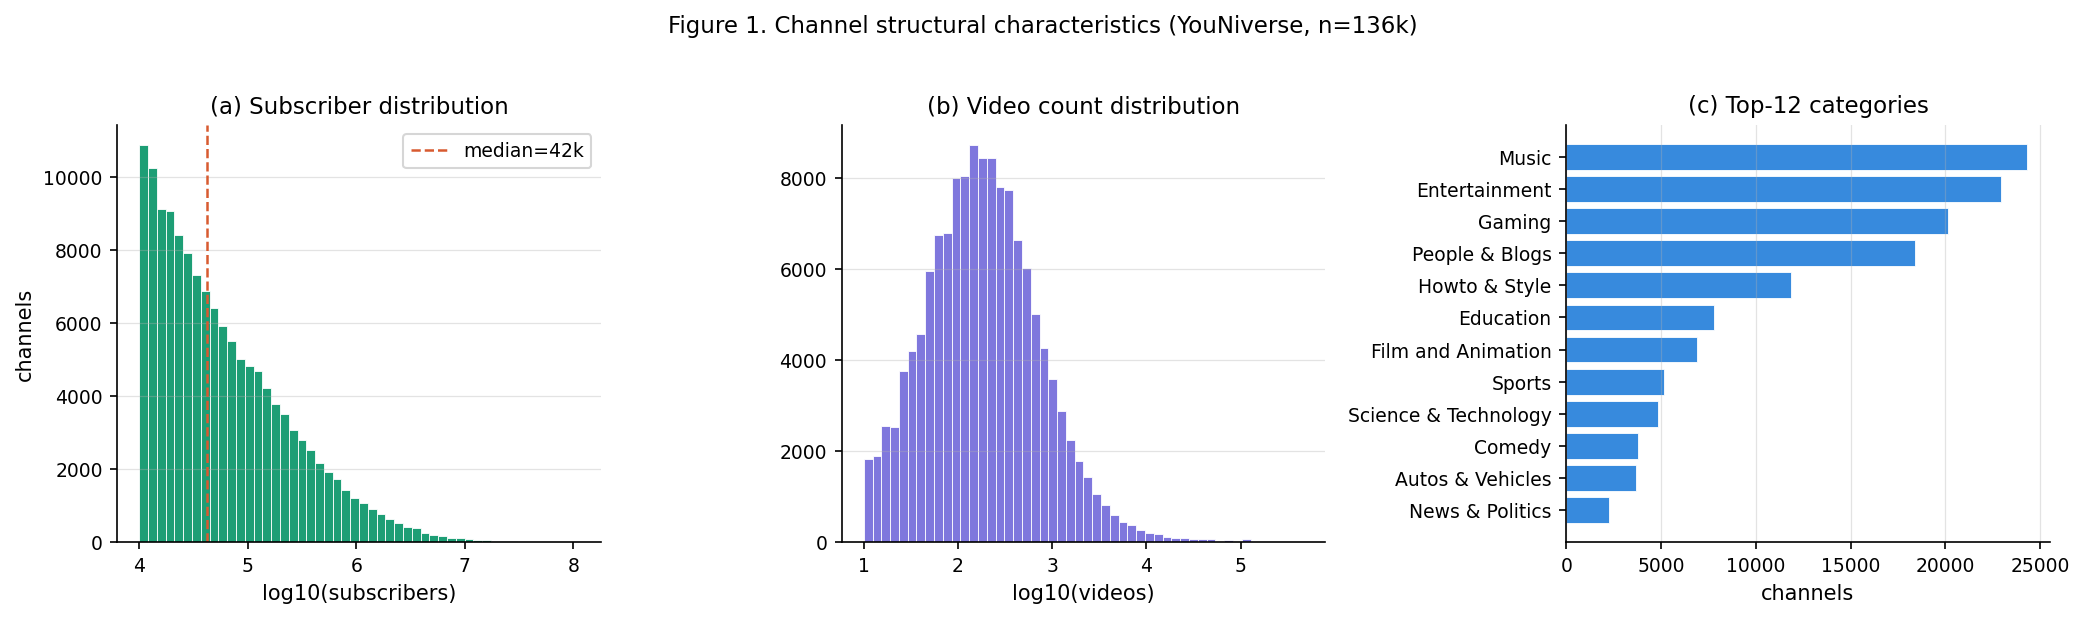
\includegraphics[width=\textwidth]{figures/Fig01_channel_structure.png}
\caption{Channel structural characteristics ($n = 136{,}470$).
(a)~Log$_{10}$-transformed subscriber distribution (median = 42k).
(b)~Log$_{10}$-transformed video count distribution.
(c)~Distribution across the top-12 content categories.
\label{fig:channels}}
\end{figure}

\begin{figure}[H]
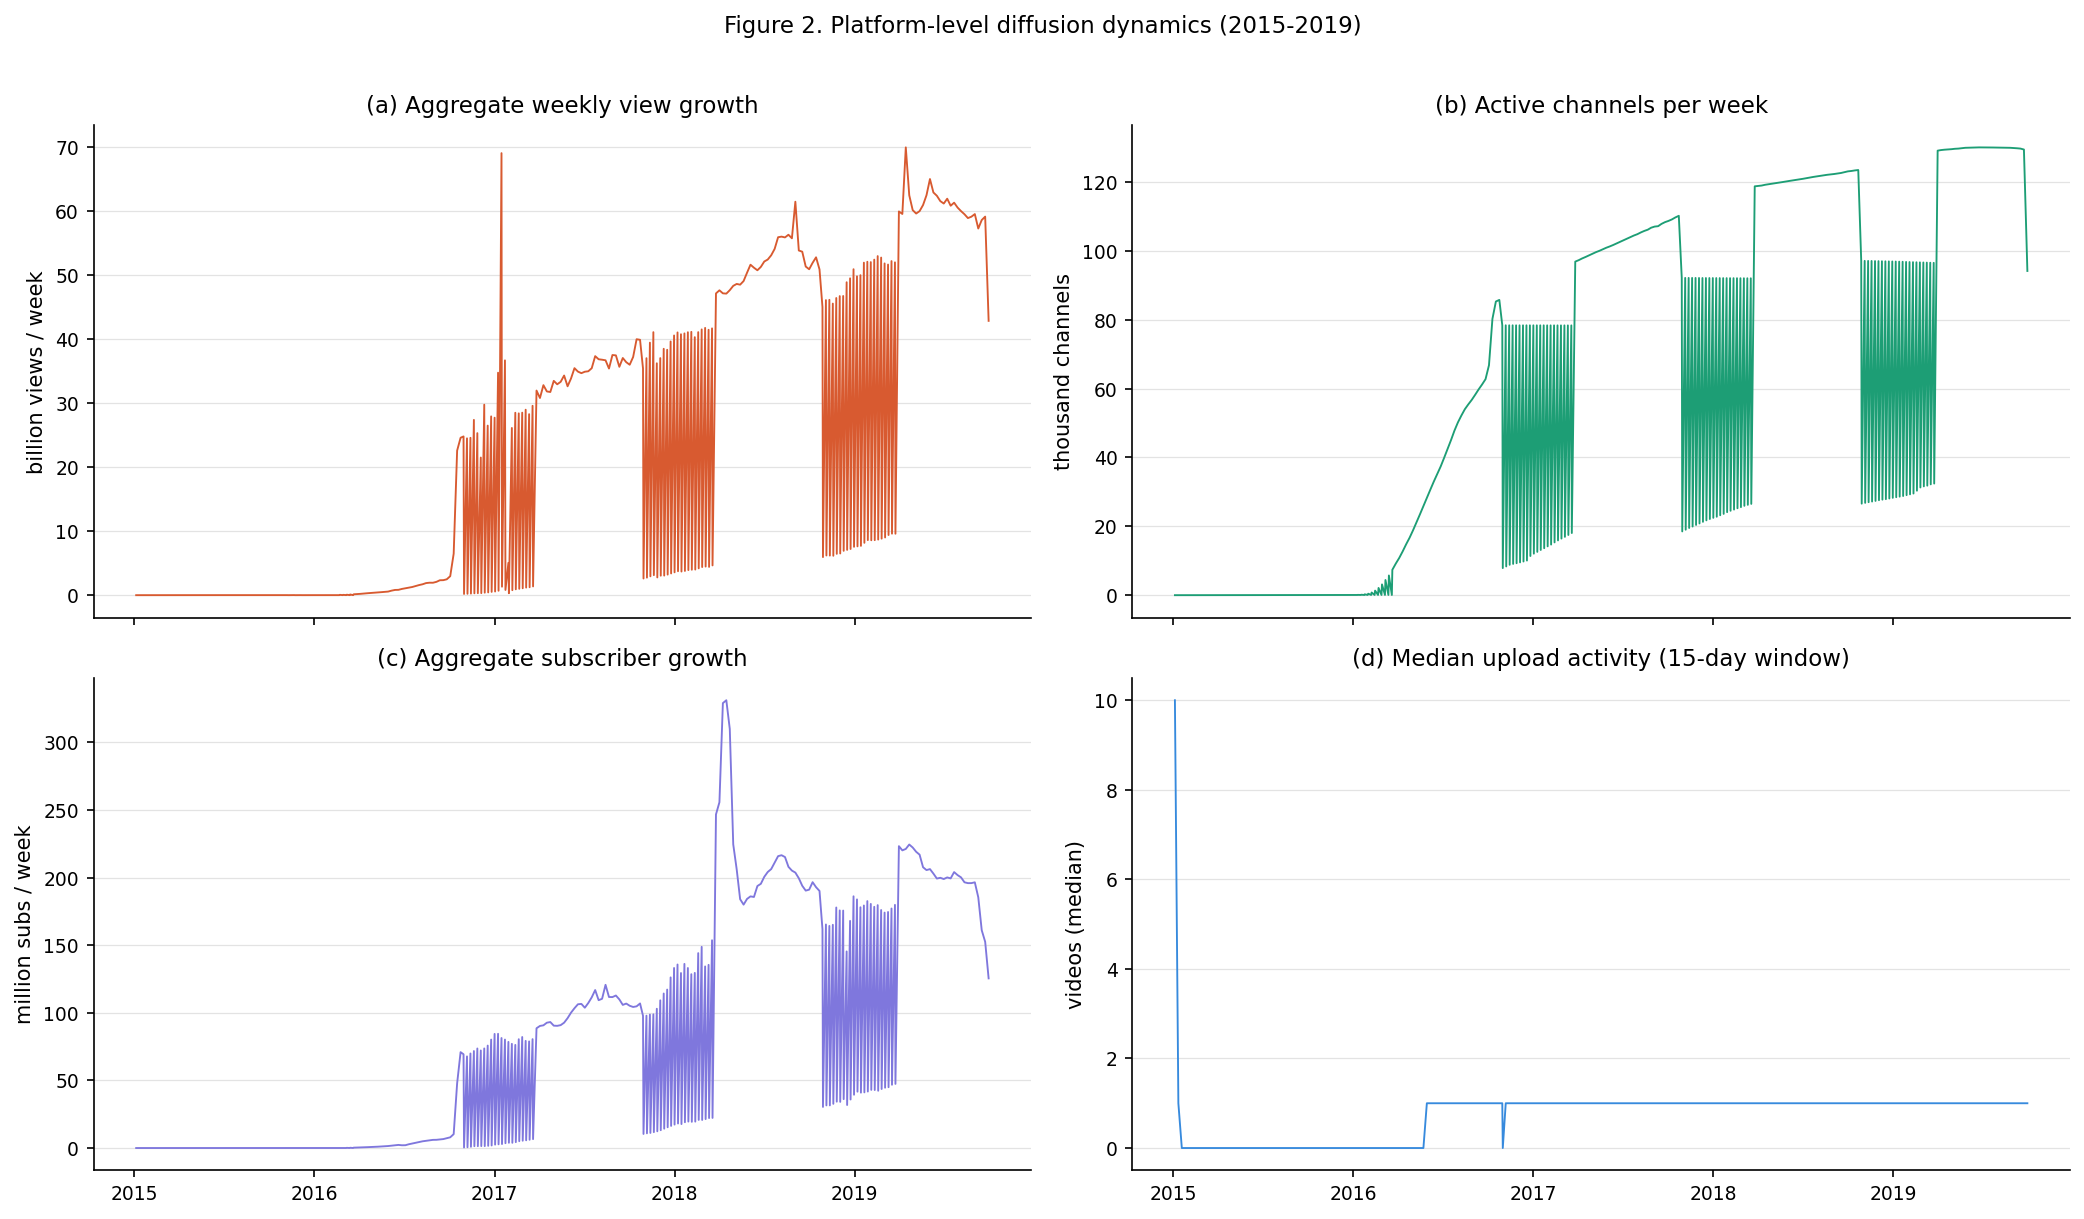
\includegraphics[width=\textwidth]{figures/Fig02_aggregate_dynamics.png}
\caption{Platform-level weekly dynamics (2015--2019) after
daylight-saving-time deduplication.
(a)~Aggregate weekly view growth.
(b)~Active channels per week.
(c)~Aggregate subscriber growth.
(d)~Median upload activity (15-day window).
\label{fig:aggregate}}
\end{figure}

\begin{figure}[H]
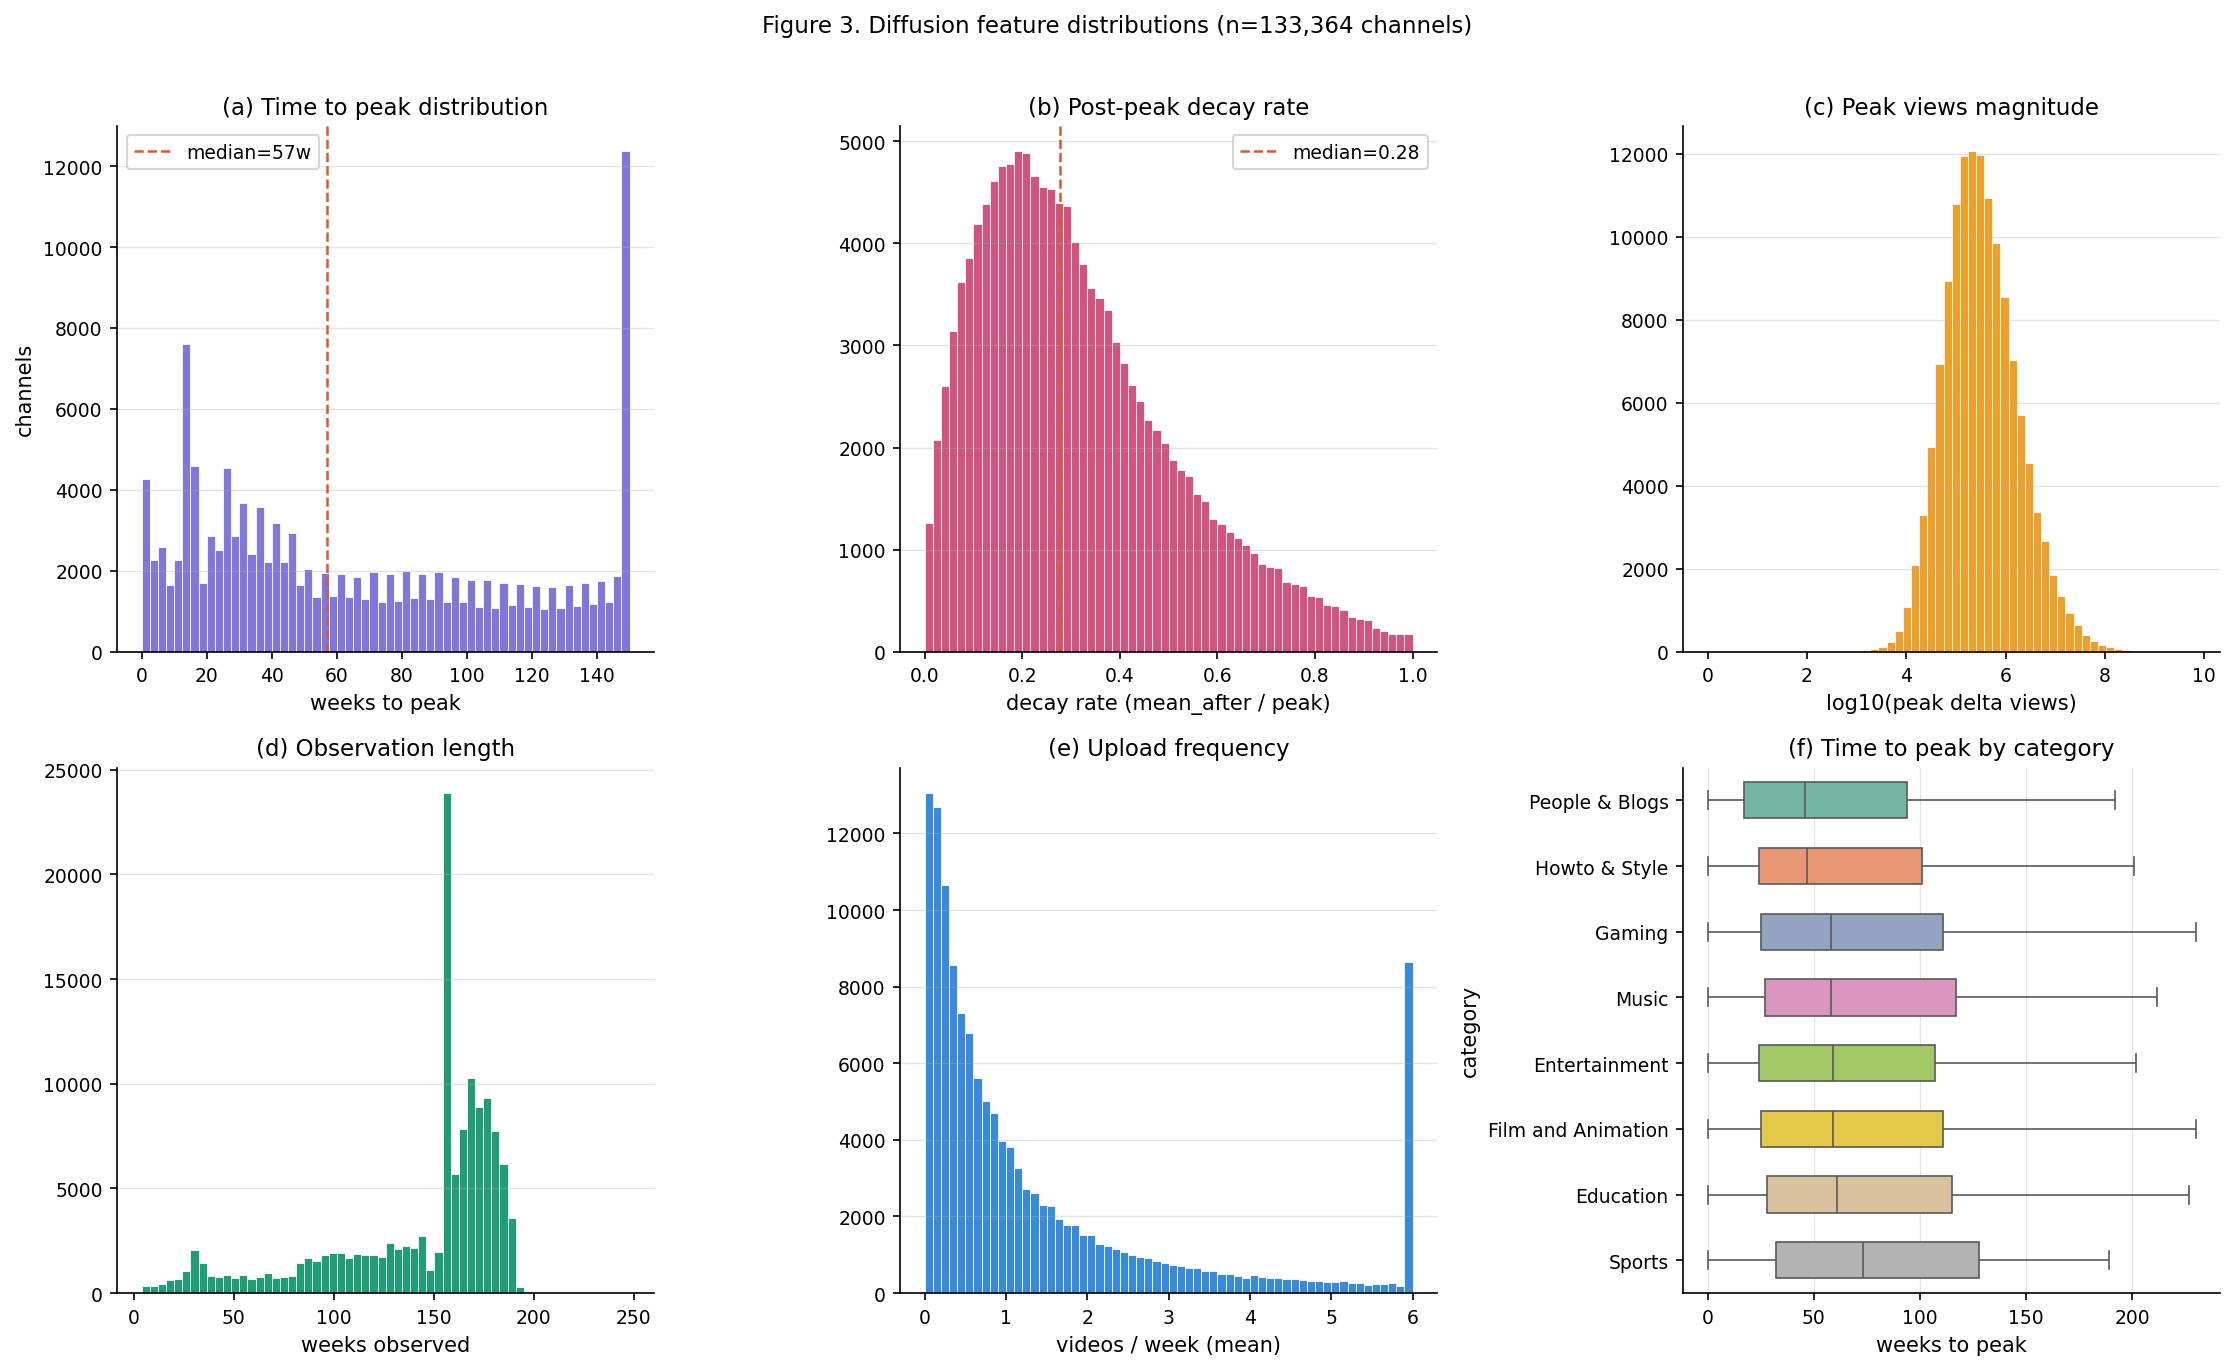
\includegraphics[width=\textwidth]{figures/Fig03_diffusion_features.png}
\caption{Distributions of derived diffusion features
($n = 133{,}364$ channels).
(a)~Time-to-peak (median = 57 weeks).
(b)~Post-peak decay rate (median = 0.277).
(c)~Peak views in log$_{10}$ scale.
(d)~Observation length.
(e)~Upload frequency.
(f)~Time-to-peak by content category (top-8; boxes show IQR).
\label{fig:diffusion}}
\end{figure}

\begin{figure}[H]
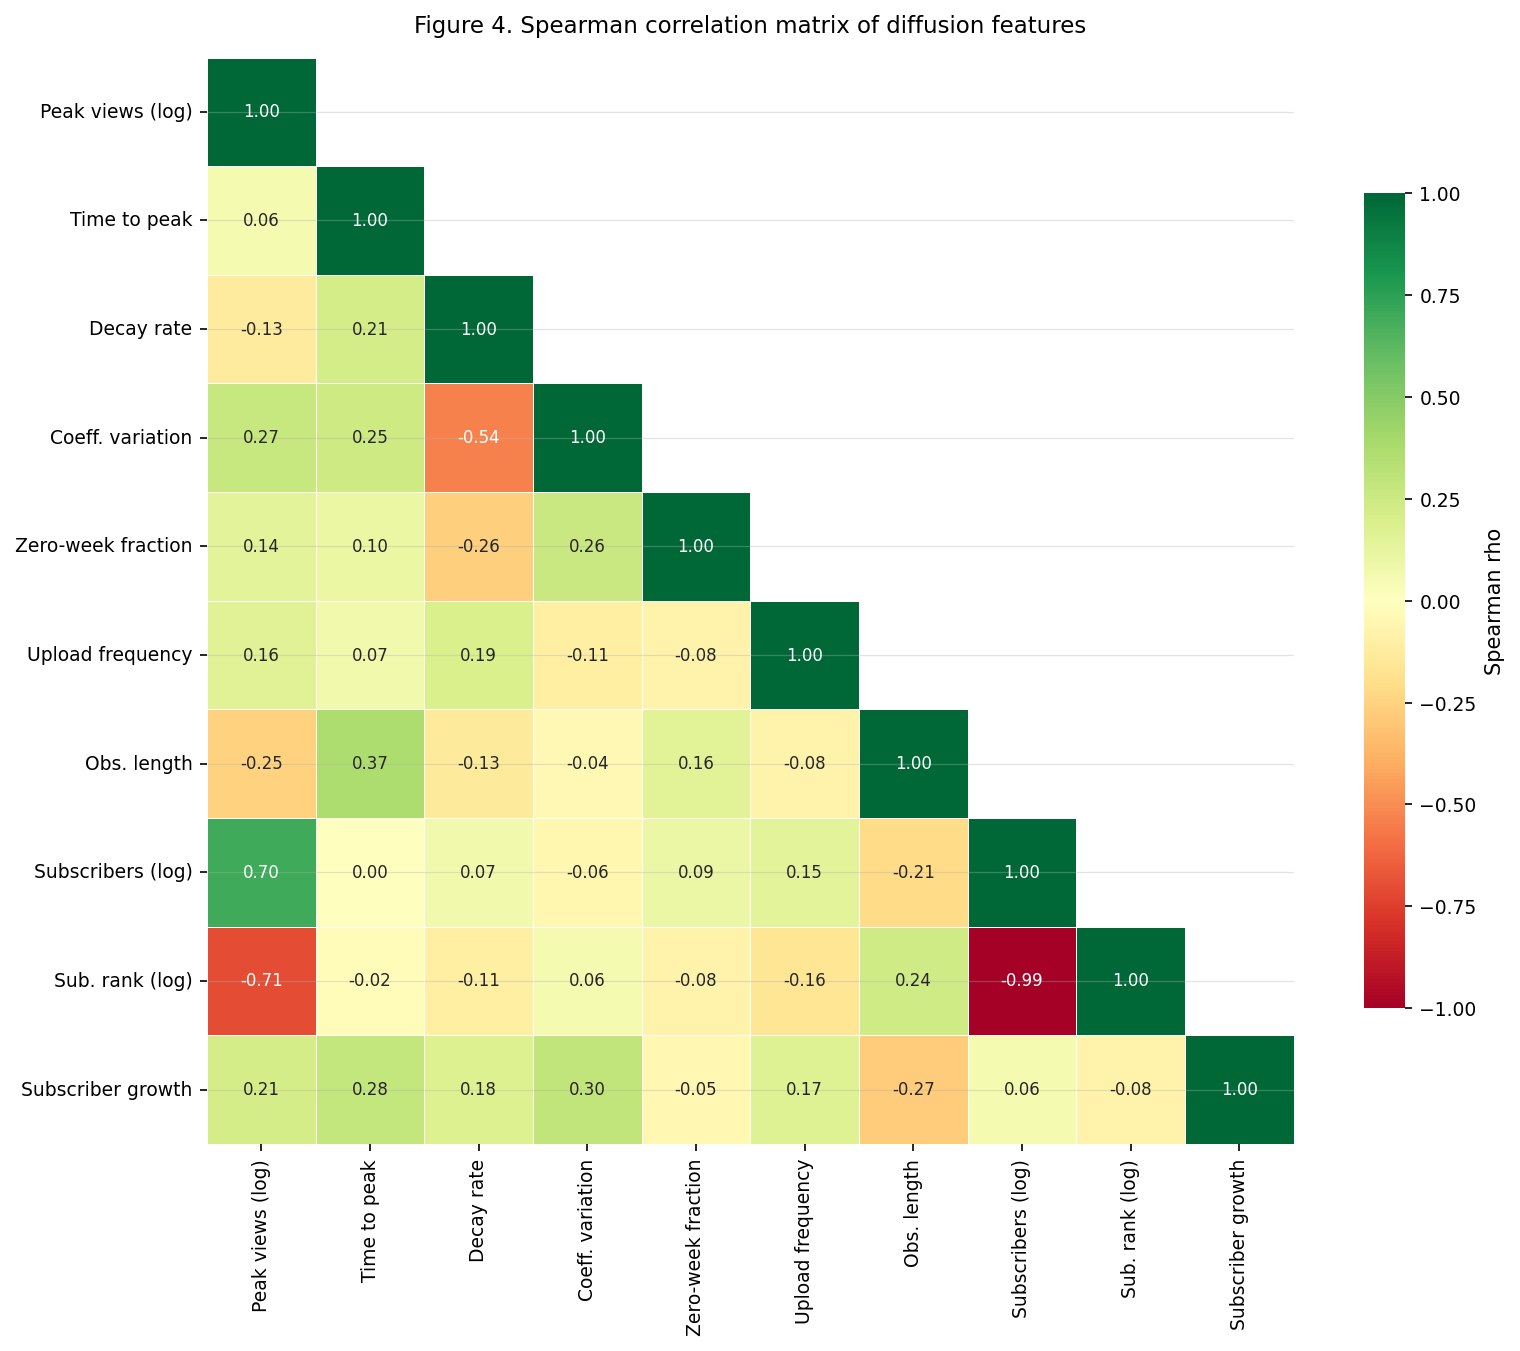
\includegraphics[width=\textwidth]{figures/Fig04_correlation_matrix.png}
\caption{Spearman correlation matrix for diffusion and structural features.
log\_subs and log\_rank are near-perfectly collinear ($\rho = -0.994$).
Time-to-peak has near-zero correlation with the regression target
($\rho = 0.056$).
\label{fig:corr}}
\end{figure}

\begin{figure}[H]
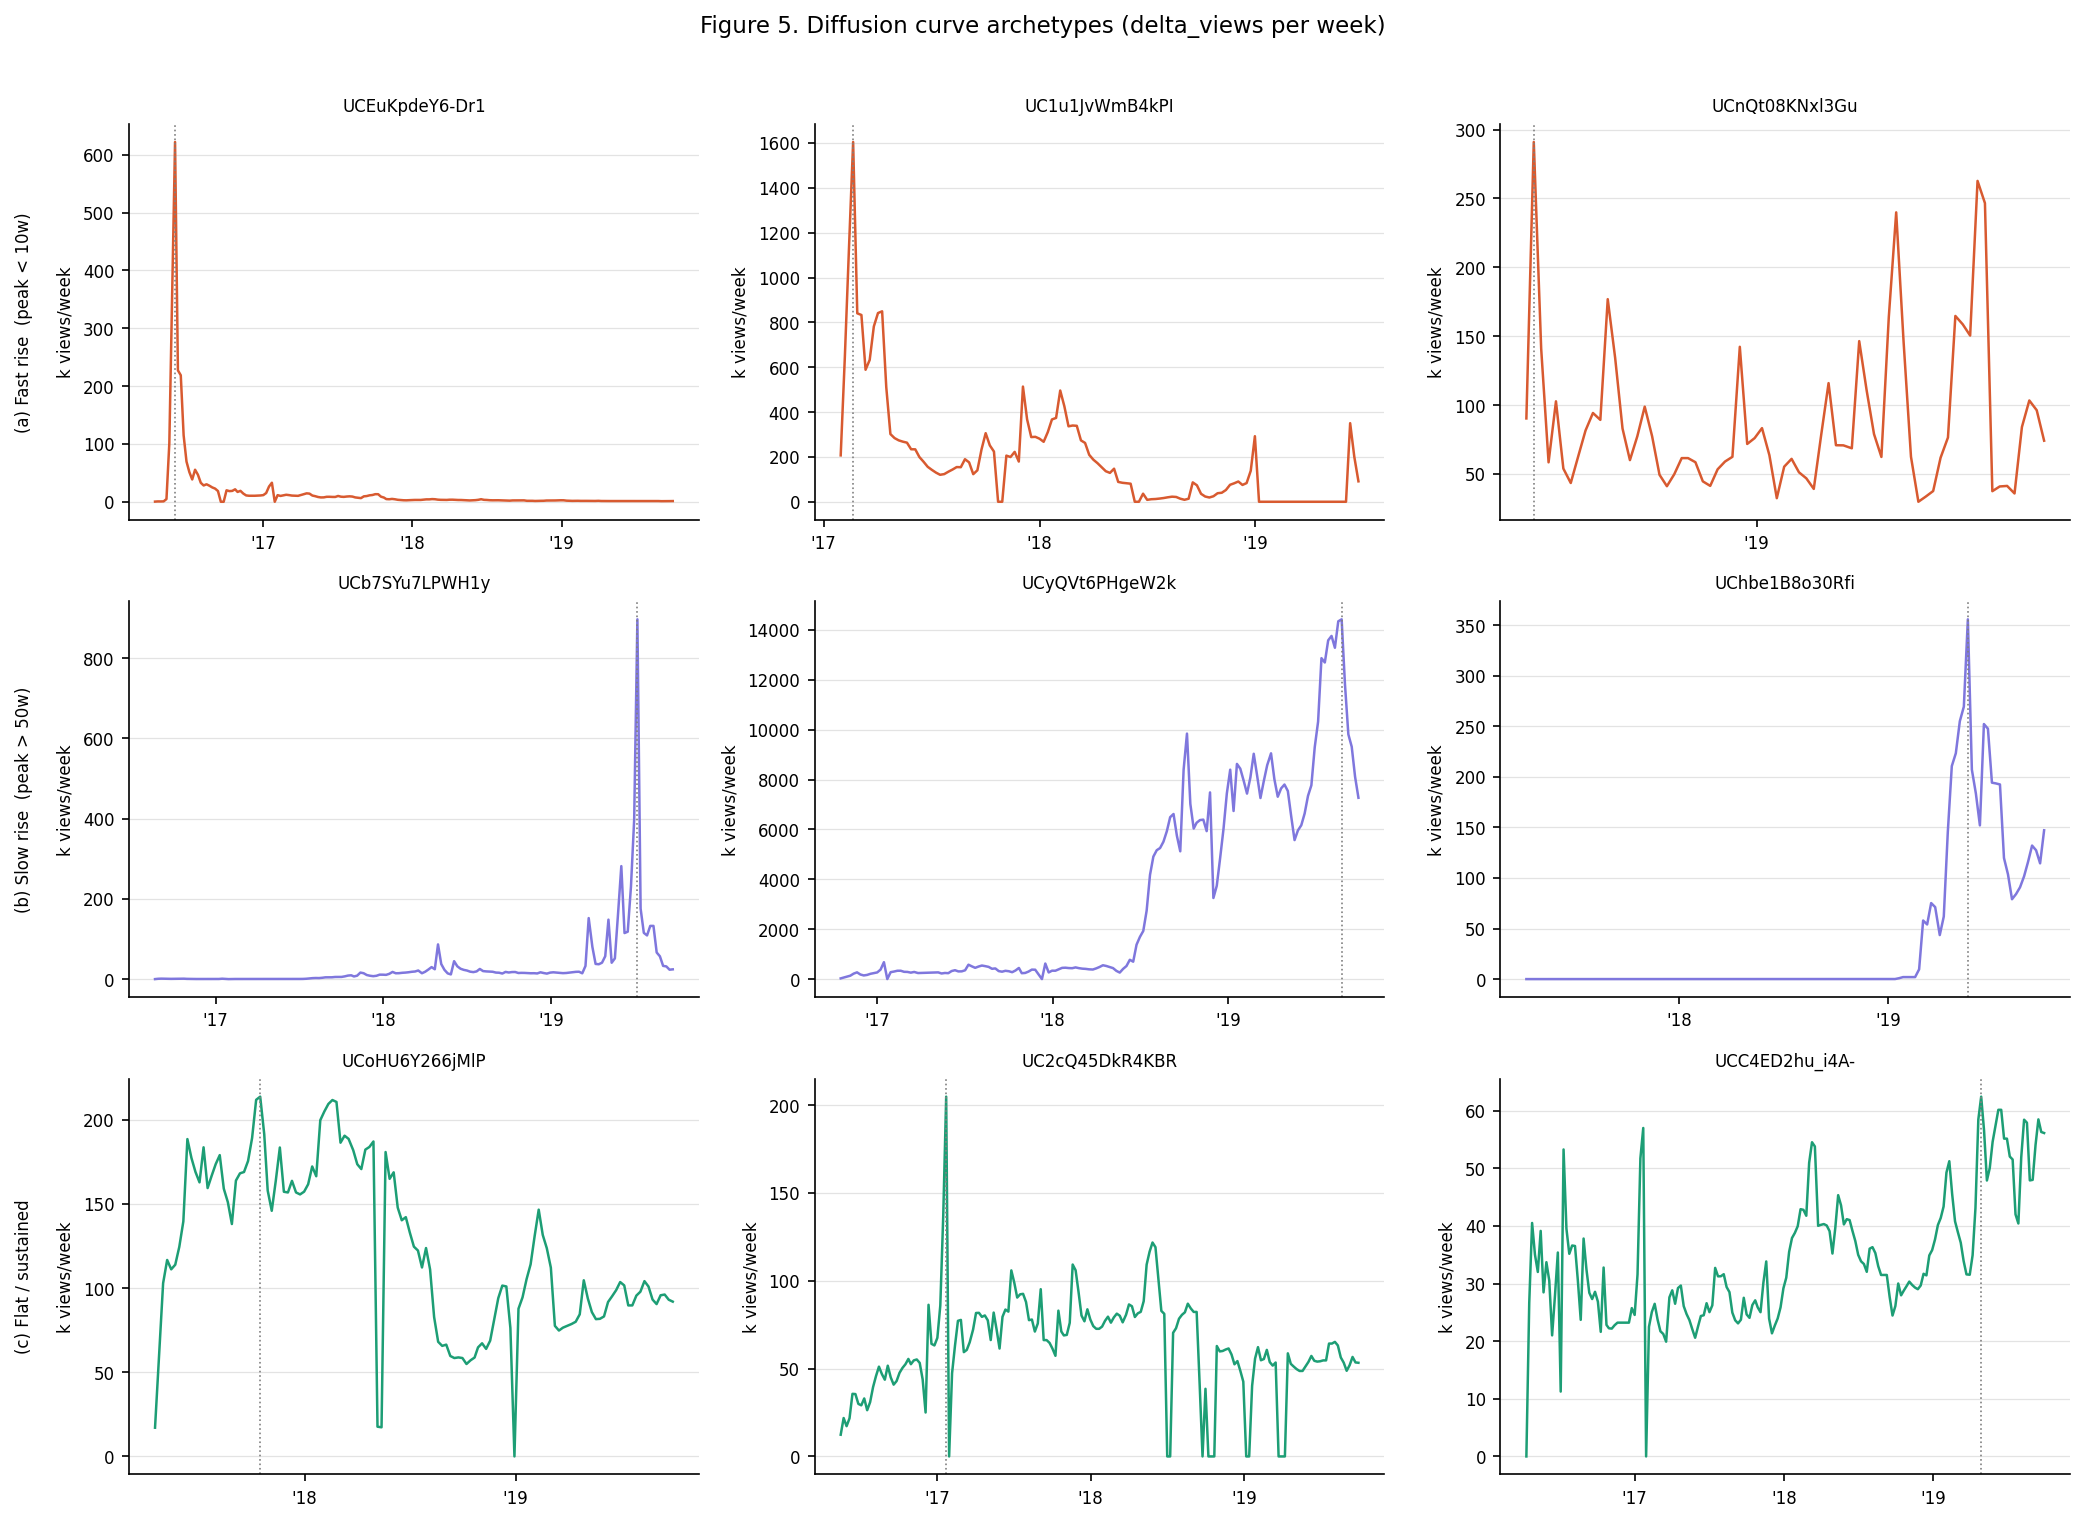
\includegraphics[width=\textwidth]{figures/Fig05_diffusion_archetypes.png}
\caption{Diffusion curve archetypes (weekly $\Delta$views).
(a)~Fast-rise channels (peak $<$ 10~weeks).
(b)~Slow-rise channels (peak $>$ 50~weeks).
(c)~Flat/sustained channels (CV $<$ 0.5).
Dashed vertical lines mark the peak week.
\label{fig:archetypes}}
\end{figure}

\begin{figure}[H]
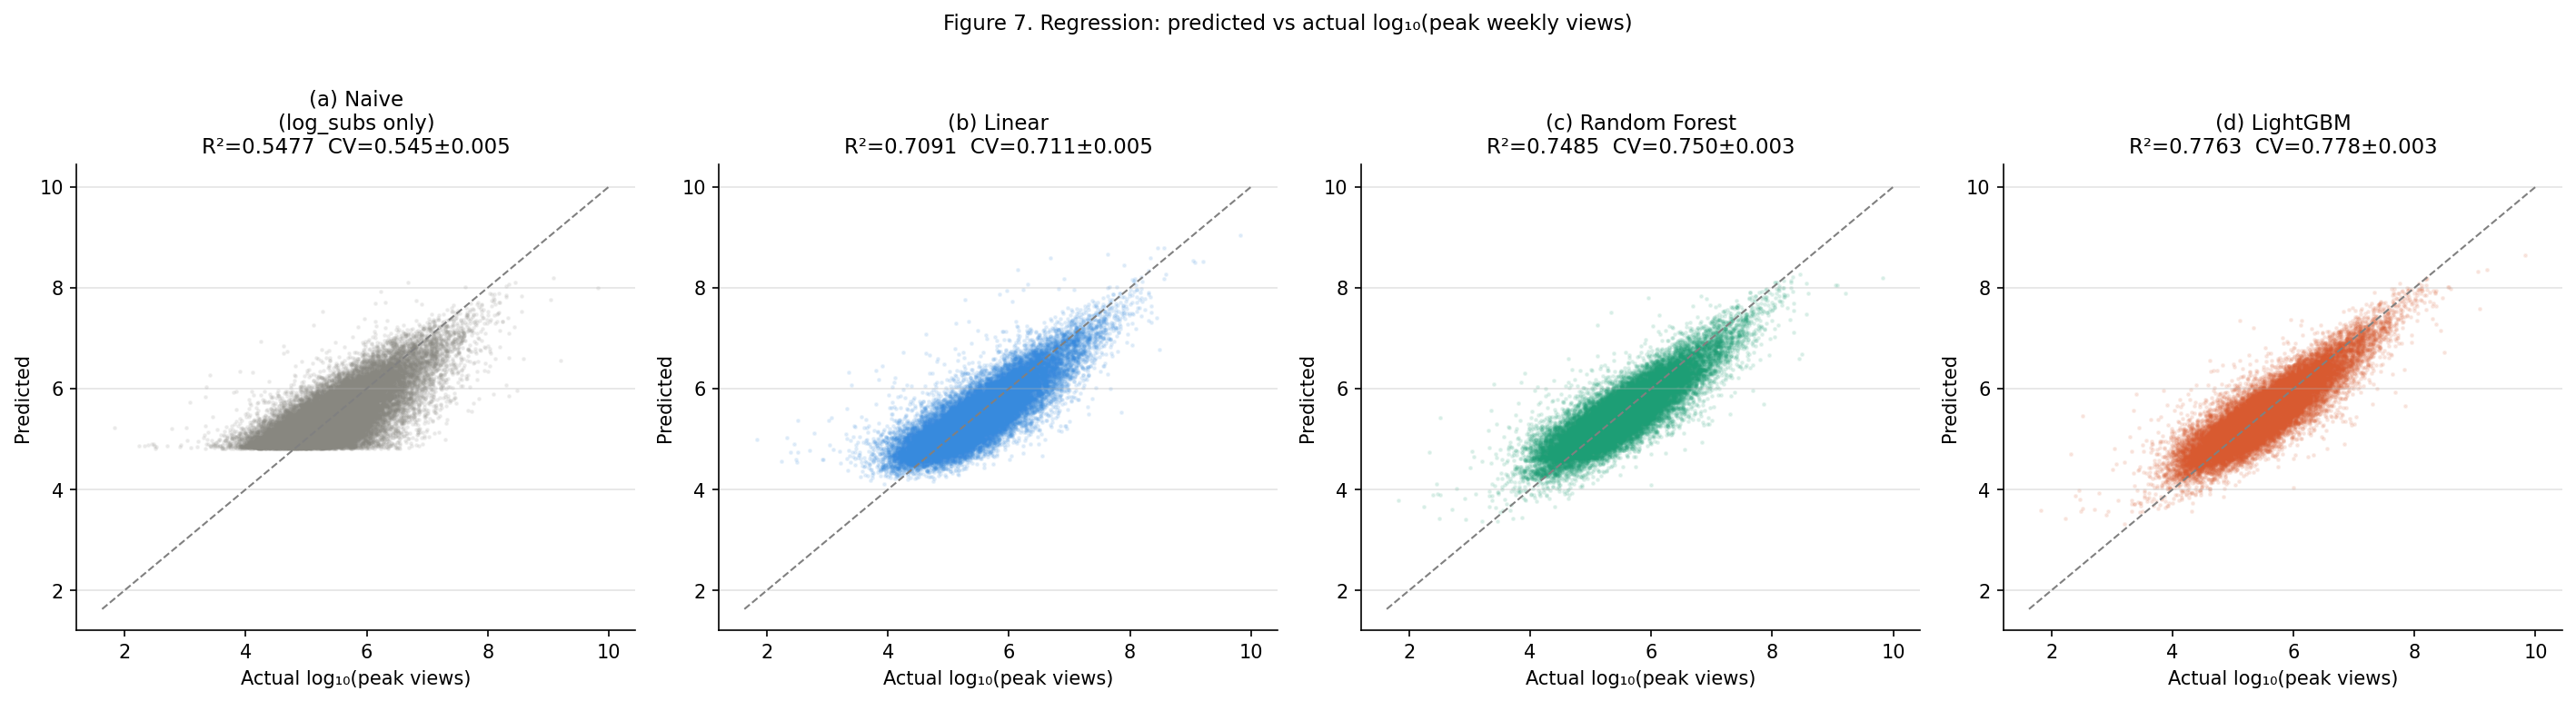
\includegraphics[width=\textwidth]{figures/Fig07_regression_predicted_vs_actual.png}
\caption{Regression: predicted vs.\ actual $\log_{10}(\Delta v_\text{peak})$
on the held-out test set.
(a)~Naive baseline (log\_subs only; $R^2 = 0.548$).
(b)~Linear Regression ($R^2 = 0.709$).
(c)~Random Forest ($R^2 = 0.749$).
(d)~LightGBM ($R^2 = 0.776$).
Dashed diagonal = perfect prediction.
CV mean~$\pm$~std shown in each panel.
\label{fig:regression}}
\end{figure}

\begin{figure}[H]
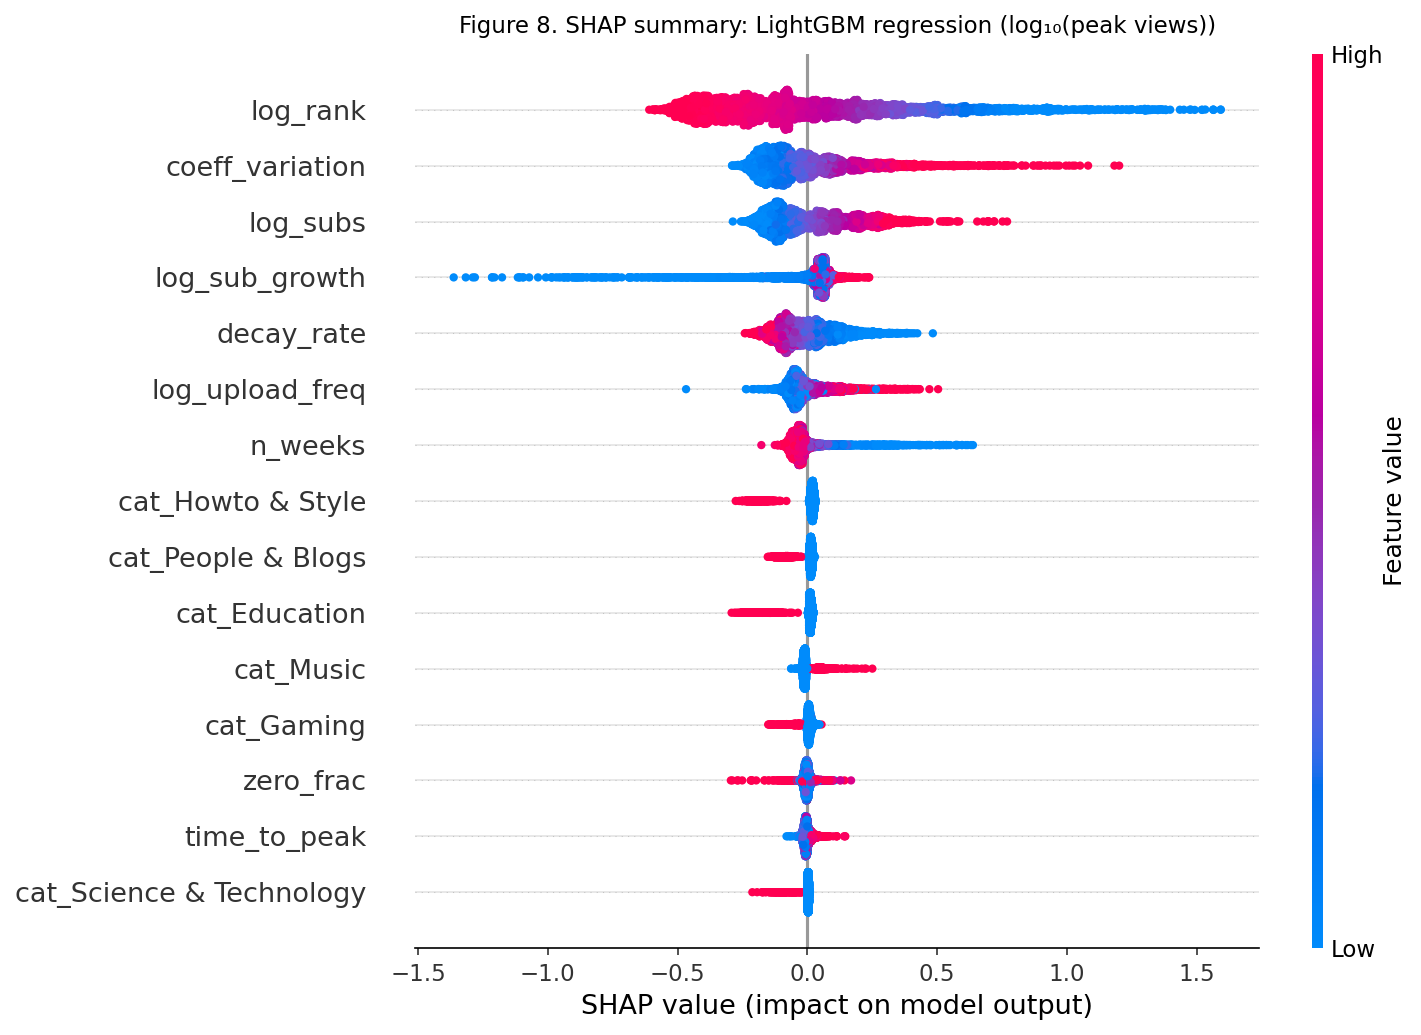
\includegraphics[width=\textwidth]{figures/Fig08_feature_importance_shap.png}
\caption{SHAP summary plot for LightGBM regression
(5,000-sample subsample of test set, top-15 features).
Each row is a feature; each point is a channel.
Colour encodes feature value (red = high, blue = low).
Horizontal axis encodes SHAP contribution to
$\hat{y} = \log_{10}(\Delta v_\text{peak})$.
log\_rank accounts for 29.3\% of total mean absolute SHAP;
time\_to\_peak ranks 14th (1.1\%).
\label{fig:shap}}
\end{figure}

\begin{figure}[H]
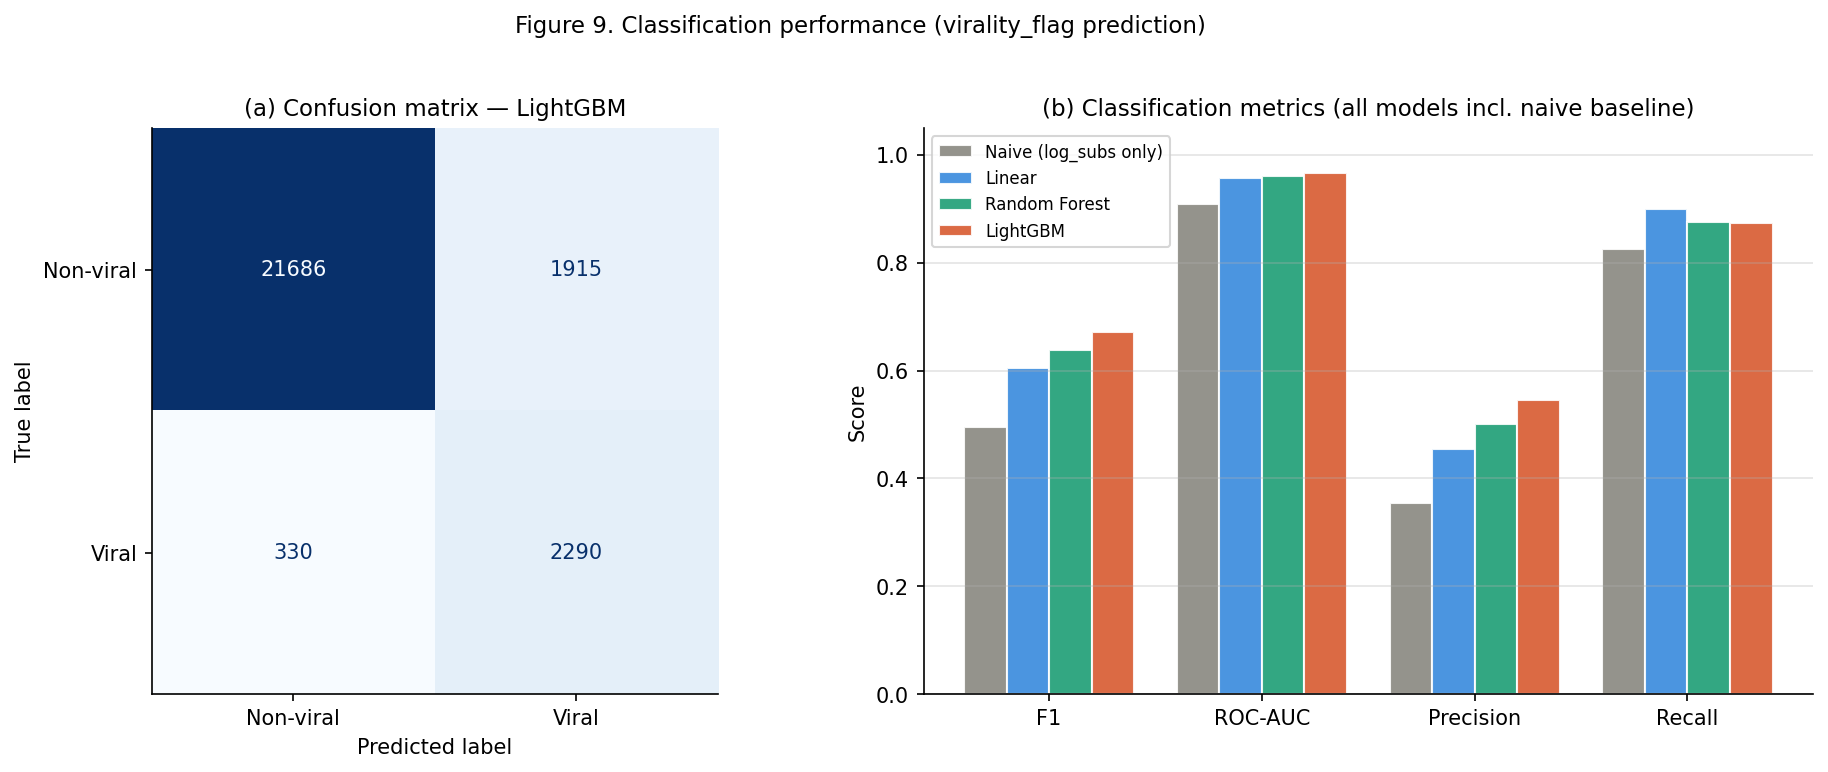
\includegraphics[width=\textwidth]{figures/Fig09_classification_results.png}
\caption{Classification performance (virality\_flag = top-10\% peak
within category).
(a)~Confusion matrix for LightGBM.
(b)~F1, ROC-AUC, Precision, Recall for all four models including the
naive baseline.
\label{fig:classification}}
\end{figure}

\begin{figure}[H]
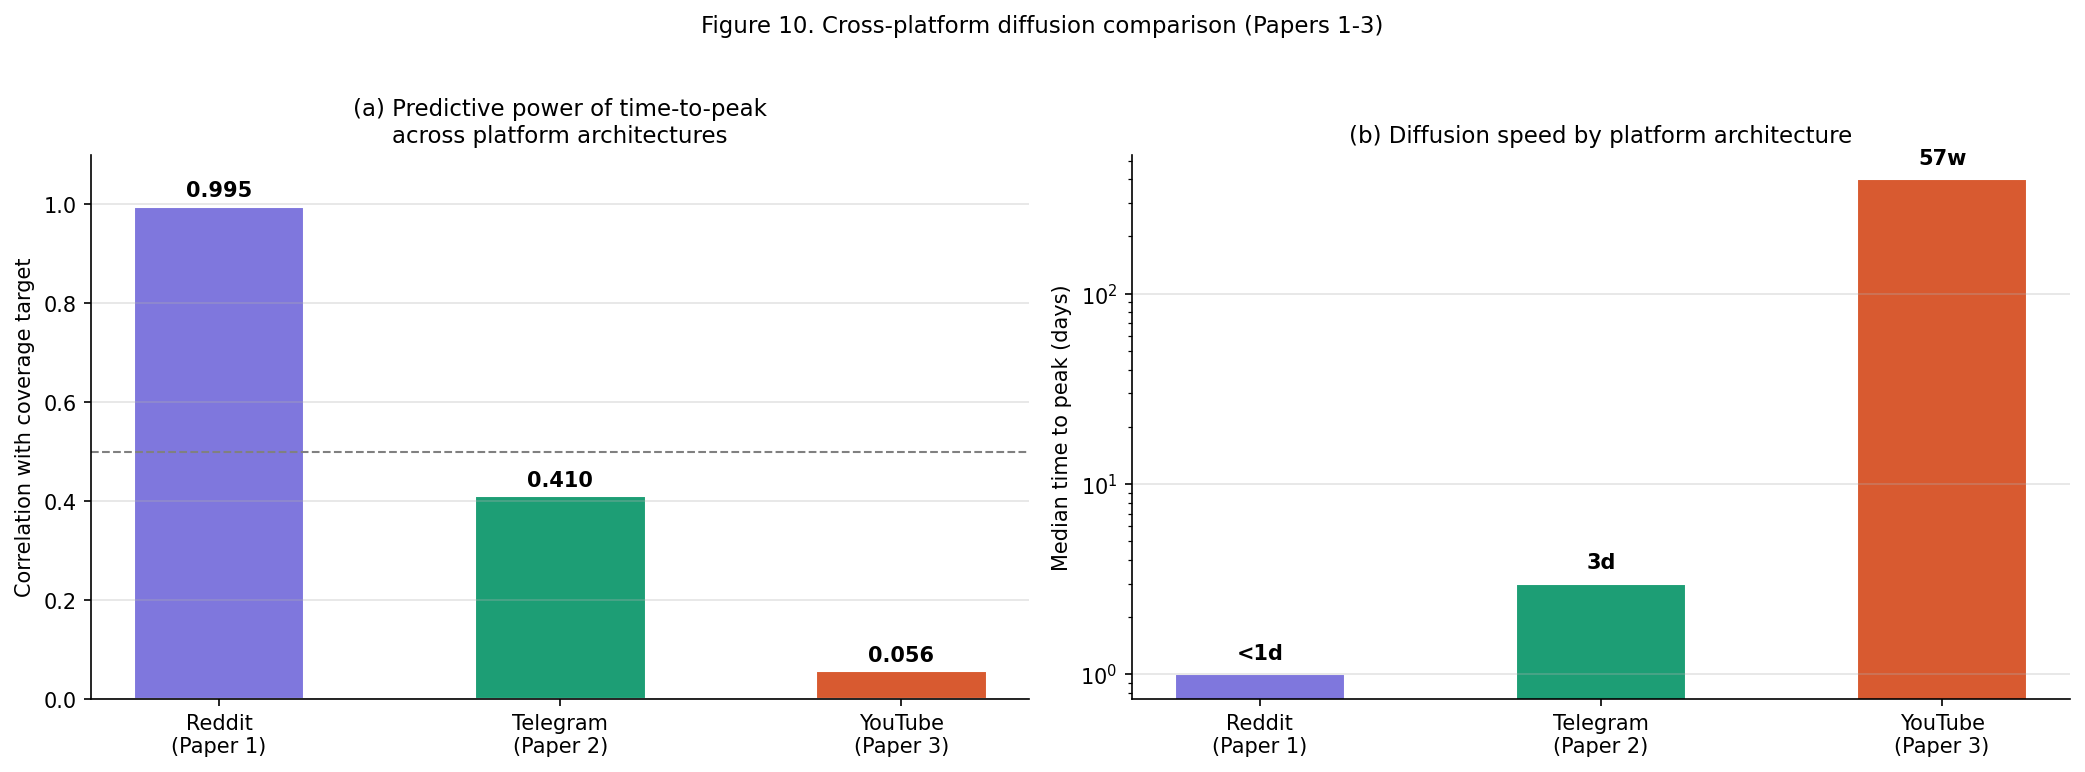
\includegraphics[width=\textwidth]{figures/Fig10_crossplatform_comparison.png}
\caption{Cross-platform comparison.
(a)~Bivariate association of time-to-peak with coverage target.
(b)~Median time-to-peak (log scale).
\label{fig:crossplatform}}
\end{figure}

\begin{figure}[H]
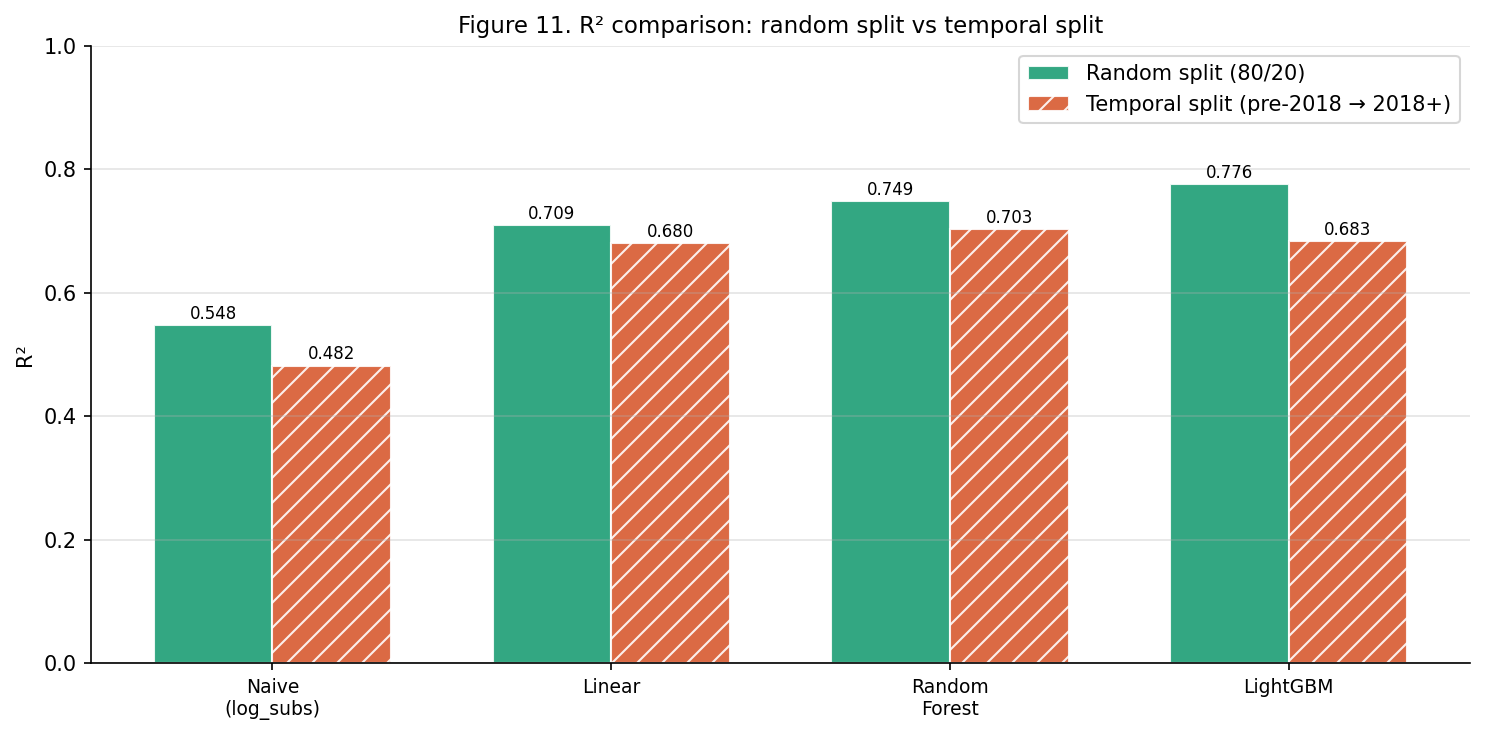
\includegraphics[width=\textwidth]{figures/Fig11_temporal_split_comparison.png}
\caption{$R^2$ comparison: random split (teal) vs.\ temporal split
(hatched coral; train on pre-2018 channels, test on 2018--2019).
Note the rank reversal: Random~Forest ($R^2 = 0.703$) outperforms
LightGBM ($R^2 = 0.683$) under the temporal split, indicating superior
cross-temporal robustness.
\label{fig:temporal}}
\end{figure}

%=================================================================
% ── Tables ───────────────────────────────────────────────────────

\begin{table}[H]
\caption{Missing-value rates after DST deduplication.\label{tab:missing}}
\begin{tabularx}{\textwidth}{llll}
\toprule
\textbf{File} & \textbf{Column} & \textbf{Missing ($n$)} & \textbf{(\%)} \\
\midrule
df\_channels\_en   & category\_cc & 128    & 0.09 \\
df\_channels\_en   & name\_cc     & 10     & 0.01 \\
df\_timeseries\_en & category     & 20,584 & 0.11 \\
\bottomrule
\end{tabularx}
\end{table}

\begin{table}[H]
\caption{Channel metadata descriptive statistics
($n = 136{,}470$).\label{tab:channels}}
\begin{tabularx}{\textwidth}{lllllll}
\toprule
\textbf{Metric}&\textbf{Mean}&\textbf{Std}&\textbf{Min}&
\textbf{P25}&\textbf{P50}&\textbf{Max}\\
\midrule
Subscribers & 246,602 & 1,150,096 & 10,000 & 18,886 & 42,400 & 112,139,463 \\
Videos      & 700     & 4,525     & 10     & 70     & 175    & 461,923 \\
Sub.\ rank  & 357,009 & 271,114   & 3      & 116,131& 301,567& 1,030,844 \\
\bottomrule
\end{tabularx}
\end{table}

\begin{table}[H]
\caption{Time-series dataset overview after preprocessing.\label{tab:ts}}
\begin{tabularx}{\textwidth}{ll}
\toprule
\textbf{Metric} & \textbf{Value} \\
\midrule
Total rows (clean)        & 18,872,499 \\
Unique channels           & 133,516 \\
Mean weeks per channel    & 141.4 \\
Median weeks per channel  & 156.0 \\
P5--P95                   & 35--185 weeks \\
Period                    & 2015-01-05 to 2019-09-30 \\
\bottomrule
\end{tabularx}
\end{table}

\begin{table}[H]
\caption{Channel distribution across content categories.
\label{tab:categories}}
\begin{tabularx}{\textwidth}{lll}
\toprule
\textbf{Category} & \textbf{Channels} & \textbf{(\%)} \\
\midrule
Music               & 24,285 & 17.81 \\
Entertainment       & 22,951 & 16.83 \\
Gaming              & 20,143 & 14.77 \\
People \& Blogs     & 18,413 & 13.51 \\
Howto \& Style      & 11,875 &  8.71 \\
Education           &  7,803 &  5.72 \\
Film and Animation  &  6,875 &  5.04 \\
Sports              &  5,148 &  3.78 \\
Science \& Technology& 4,864 &  3.57 \\
Comedy              &  3,767 &  2.76 \\
Autos \& Vehicles   &  3,705 &  2.72 \\
News \& Politics    &  2,263 &  1.66 \\
Travel \& Events    &  1,989 &  1.46 \\
Pets \& Animals     &  1,292 &  0.95 \\
Nonprofits \& Activism & 969 &  0.71 \\
\bottomrule
\end{tabularx}
\end{table}

\begin{table}[H]
\caption{Diffusion feature descriptive statistics
($n = 133{,}364$).\label{tab:diffusion}}
\begin{tabularx}{\textwidth}{lllllll}
\toprule
\textbf{Feature}&\textbf{Mean}&\textbf{Std}&\textbf{Min}&
\textbf{P25}&\textbf{P50}&\textbf{Max}\\
\midrule
Time-to-peak (wk)  & 68.9  & 50.4  & 0     & 25    & 57    & 230 \\
Decay rate         & 0.317 & 0.205 & 0.000 & 0.161 & 0.277 & 1.000 \\
Coeff.\ variation  & 0.988 & 0.745 & 0.056 & 0.525 & 0.785 & 11.53$^*$ \\
Zero-week fraction & 0.026 & 0.052 & 0.000 & 0.006 & 0.011 & 1.000 \\
Upload freq (v/wk) & 2.22  & 8.59  & 0.000 & 0.268 & 0.737 & 644.1$^*$ \\
Weeks observed     & 141.5 & 43.8  & 4     & 122   & 156   & 248 \\
Peak $\Delta$views & 1,983k& 22,594k& 0    & 98k   & 284k  & 6.66B \\
Sub.\ growth       & 540.3 & 6,049 & $-0.40$& 1.58 & 8.34  & 867,499$^*$ \\
\bottomrule
\multicolumn{7}{l}{\footnotesize $^*$Clipped at the 99.9th percentile
before log$_{1}p$ transformation.}
\end{tabularx}
\end{table}

\begin{table}[H]
\caption{Feature set used in machine learning models.\label{tab:features}}
\begin{tabularx}{\textwidth}{llll}
\toprule
\textbf{Feature}&\textbf{Group}&\textbf{Description}&\textbf{Transform}\\
\midrule
time\_to\_peak     & Temporal    & Weeks to peak $\Delta$views          & None \\
decay\_rate        & Temporal    & Mean post-peak / peak views           & Clip [0,1] \\
coeff\_variation   & Temporal    & Std / mean $\Delta$views              & Clip p99.9 \\
zero\_frac         & Temporal    & Fraction zero-view weeks              & None \\
n\_weeks           & Temporal    & Total weeks observed                  & None \\
log\_upload\_freq  & Behavioural & Mean videos / week                    & $\log_{1}p$ \\
log\_subs          & Structural  & Subscribers (Oct 2019 crawl)          & $\log_{10}$ \\
log\_rank          & Structural  & Subscriber rank (Oct 2019 crawl)      & $\log_{10}$ \\
log\_sub\_growth   & Structural  & Relative subscriber growth            & $\log_{1}p$ \\
channel\_age\_days & Structural  & Days from obs.\ start to peak week   & None \\
cat\_* (14)        & Categorical & Content category dummies              & OHE \\
\bottomrule
\multicolumn{4}{l}{\footnotesize Structural features marked ``Oct 2019 crawl'' are
post-hoc for channels peaking before 2019; see Section~\ref{sec:temporal_split}.}
\end{tabularx}
\end{table}

\begin{table}[H]
\caption{Virality flag class balance ($n = 131{,}105$).\label{tab:balance}}
\begin{tabularx}{\textwidth}{lll}
\toprule
\textbf{Class}&\textbf{Count}&\textbf{Percentage}\\
\midrule
Non-viral (0) & 118,004 & 90.01\% \\
Viral (1)     &  13,101 &  9.99\% \\
\bottomrule
\end{tabularx}
\end{table}

\begin{table}[H]
\caption{Selected Spearman correlations with $\log_{10}(\Delta v_\text{peak})$.
Full matrix in Figure~\ref{fig:corr}.\label{tab:corr_selected}}
\begin{tabularx}{\textwidth}{lll}
\toprule
\textbf{Feature}&\textbf{Spearman $\rho$}&\textbf{$|\rho|$}\\
\midrule
log\_rank         & $-0.708$ & 0.708 \\
log\_subs         & $+0.703$ & 0.703 \\
coeff\_variation  & $+0.273$ & 0.273 \\
n\_weeks          & $-0.255$ & 0.255 \\
sub\_growth       & $+0.212$ & 0.212 \\
upload\_freq      & $+0.163$ & 0.163 \\
zero\_frac        & $+0.142$ & 0.142 \\
decay\_rate       & $-0.126$ & 0.126 \\
\textbf{time\_to\_peak} & $\mathbf{+0.056}$ & \textbf{0.056} \\
\midrule
\multicolumn{2}{l}{log\_subs vs.\ log\_rank collinearity:} & $\rho = -0.994$ \\
\bottomrule
\end{tabularx}
\end{table}

\begin{table}[H]
\caption{Regression results: random 80/20 split and 5-fold CV.
Target: $\log_{10}(\Delta v_\text{peak})$.\label{tab:regression}}
\begin{tabularx}{\textwidth}{lllllll}
\toprule
\textbf{Model}&\textbf{$R^2$}&\textbf{RMSE$_\text{log}$}&
\textbf{MAE$_\text{log}$}&\textbf{RMSE$_\text{views}$}&
\textbf{CV $R^2$}&\textbf{CV RMSE}\\
\midrule
Naive (log\_subs)  & 0.548 & 0.499 & 0.388 & 43.4M &
  $0.545 \pm 0.005$ & $0.500 \pm 0.002$ \\
Linear             & 0.709 & 0.400 & 0.308 & 36.9M &
  $0.711 \pm 0.005$ & $0.399 \pm 0.003$ \\
Random Forest      & 0.749 & 0.372 & 0.290 & 42.7M &
  $0.750 \pm 0.003$ & $0.371 \pm 0.001$ \\
\textbf{LightGBM}  &\textbf{0.776}&\textbf{0.351}&\textbf{0.270}& 40.9M &
  $\mathbf{0.778 \pm 0.003}$ & $\mathbf{0.349 \pm 0.002}$ \\
\midrule
Gain vs.\ Naive (LGB) & $+0.228$ & $-0.148$ & $-0.118$ & & & \\
\bottomrule
\multicolumn{7}{l}{\footnotesize RMSE$_\text{views}$: dominated by channels
with peak $> 10^8$ weekly views; RMSE$_\text{log}$ is the primary metric.}
\end{tabularx}
\end{table}

\begin{table}[H]
\caption{Classification results: random split and 5-fold stratified CV.
Target: virality\_flag.\label{tab:classification}}
\begin{tabularx}{\textwidth}{lllllll}
\toprule
\textbf{Model}&\textbf{F1}&\textbf{ROC-AUC}&\textbf{Prec.}&
\textbf{Recall}&\textbf{CV F1}&\textbf{CV AUC}\\
\midrule
Naive (log\_subs) & 0.496 & 0.909 & 0.355 & 0.826 &
  $0.495 \pm 0.004$ & $0.908 \pm 0.005$ \\
Linear            & 0.604 & 0.957 & 0.455 & 0.899 &
  $0.603 \pm 0.004$ & $0.957 \pm 0.001$ \\
Random Forest     & 0.638 & 0.961 & 0.502 & 0.876 &
  $0.637 \pm 0.004$ & $0.960 \pm 0.002$ \\
\textbf{LightGBM} &\textbf{0.671}&\textbf{0.967}& 0.545 & 0.874 &
  $\mathbf{0.668 \pm 0.002}$ & $\mathbf{0.966 \pm 0.001}$ \\
\bottomrule
\end{tabularx}
\end{table}

\begin{table}[H]
\caption{Feature importance: LightGBM gain (T16) vs.\ SHAP mean
absolute attribution (T16b), top-10 by SHAP rank.\label{tab:importance}}
\begin{tabularx}{\textwidth}{lllll}
\toprule
\textbf{SHAP rank}&\textbf{Feature}&\textbf{Gain rank}&
\textbf{Gain (\%)}&\textbf{SHAP (\%)}\\
\midrule
1  & log\_rank          & 9  &  7.8 & \textbf{29.3} \\
2  & coeff\_variation   & 3  & 11.5 & 13.7 \\
3  & log\_subs          & 7  &  8.0 & 12.9 \\
4  & log\_sub\_growth   & 2  & 12.0 &  8.9 \\
5  & decay\_rate        & 4  & 10.3 &  8.3 \\
6  & log\_upload\_freq  & \textbf{1} & \textbf{12.6} & 6.1 \\
7  & n\_weeks           & 5  & 10.0 &  5.4 \\
8  & cat\_Howto\&Style  & 13 &  1.1 &  3.2 \\
9  & cat\_People\&Blogs & 15 &  0.9 &  2.3 \\
10 & cat\_Education     & 14 &  0.9 &  2.0 \\
\midrule
\textbf{14} & \textbf{time\_to\_peak} & 8  & 7.9 & \textbf{1.1} \\
\bottomrule
\multicolumn{5}{l}{\footnotesize Ranks 11--13 are content category dummies.
SHAP is the primary interpretability metric (see Section~\ref{sec:importance}).}
\end{tabularx}
\end{table}

\begin{table}[H]
\caption{LightGBM regression $R^2$ stratified by content category
(held-out test set; categories with $n < 20$ excluded).\label{tab:category}}
\begin{tabularx}{\textwidth}{lllll}
\toprule
\textbf{Category}&\textbf{$n$}&\textbf{$R^2$}&
\textbf{F1}&\textbf{AUC}\\
\midrule
Pets \& Animals         &   267 & 0.846 & 0.710 & 0.977 \\
Howto \& Style          & 2,293 & 0.831 & 0.652 & 0.971 \\
News \& Politics        &   459 & 0.814 & 0.752 & 0.974 \\
Sports                  &   991 & 0.810 & 0.717 & 0.977 \\
Education               & 1,515 & 0.803 & 0.665 & 0.967 \\
Entertainment           & 4,420 & 0.801 & 0.717 & 0.973 \\
Film and Animation      & 1,330 & 0.777 & 0.682 & 0.973 \\
Comedy                  &   747 & 0.775 & 0.718 & 0.969 \\
Science \& Technology   &   907 & 0.771 & 0.689 & 0.967 \\
Autos \& Vehicles       &   734 & 0.740 & 0.735 & 0.972 \\
Gaming                  & 3,829 & 0.736 & 0.651 & 0.966 \\
Music                   & 4,627 & 0.736 & 0.668 & 0.966 \\
Travel \& Events        &   398 & 0.730 & 0.653 & 0.975 \\
People \& Blogs         & 3,515 & 0.716 & 0.616 & 0.952 \\
Nonprofits \& Activism  &   189 & 0.678 & 0.571 & 0.928 \\
\bottomrule
\multicolumn{5}{l}{\footnotesize Note: best-predicted categories are
not the largest; internal heterogeneity of Music ($n = 4{,}627$) and
Gaming ($n = 3{,}829$) reduces predictive accuracy.}
\end{tabularx}
\end{table}

\begin{table}[H]
\caption{Temporal split regression results (train: peak $<$ 2018,
$n = 51{,}084$; test: peak $\geq$ 2018, $n = 80{,}021$).\label{tab:temporal}}
\begin{tabularx}{\textwidth}{lllll}
\toprule
\textbf{Model}&\textbf{$R^2$ (random)}&\textbf{$R^2$ (temporal)}&
\textbf{Drop (pp)}&\textbf{RMSE$_\text{log}$ (temporal)}\\
\midrule
Naive (log\_subs)  & 0.548 & 0.482 & $-6.6$ & 0.530 \\
Linear             & 0.709 & 0.681 & $-2.8$ & 0.416 \\
\textbf{Random Forest} & 0.749 & \textbf{0.703} & $-4.6$ & \textbf{0.401} \\
LightGBM           & 0.776 & 0.683 & $-9.3$ & 0.414 \\
\bottomrule
\multicolumn{5}{l}{\footnotesize Rank reversal under temporal split:
RF ($R^2 = 0.703$) $>$ LightGBM ($R^2 = 0.683$). LightGBM's larger
drop (9.3~pp) reflects greater sensitivity to distributional shift.}
\end{tabularx}
\end{table}

\begin{table}[H]
\caption{Cross-platform comparison across the three studies in this
series.\label{tab:crossplatform}}
\begin{tabularx}{\textwidth}{llll}
\toprule
\textbf{Property}&\textbf{Reddit~\cite{ref-paper1}}&
\textbf{Telegram~\cite{ref-paper2}}&\textbf{YouTube (this study)}\\
\midrule
Platform type  & Graph (thread cascades) & Broadcast (star, depth=1) &
  Algorithmic recommendation \\
Dataset        & Synth.\ + real threads  & 5,000+ cascades &
  133,364 ch., 18.9M obs. \\
Best model     & Gradient Boosting & Delay-driven star & LightGBM \\
Temporal robust & N/A & N/A &
  \textbf{RF beats LightGBM} \\
Best metric    & $R^2 = 0.847$ & Med.\ error $<$ 10\% &
  $R^2 = 0.776$; AUC = 0.967 \\
Naive $R^2$    & N/A & N/A & 0.548 \\
Model gain     & N/A & N/A & $\Delta R^2 = +0.228$ \\
Median TTP     & Hours--days & Days & 57 weeks \\
TTP bivariate  & $r = 0.995$ & Partial & $\rho = 0.056$ \\
TTP SHAP rank  & \#1 & N/A & \#14 (1.1\%) \\
Top SHAP feat. & peak\_speed\_time & Delay distribution &
  log\_rank (29.3\%) \\
\bottomrule
\end{tabularx}
\end{table}

\PublishersNote{}
\end{adjustwidth}
\end{document}
